%%%%%%%%%%%%%%%%%%%%%%%%%%%%%%%%%%%
%%%  Filename: thesis_template.tex
%%%  ---
%%%  Template for Master Thesis at DTETI UGM   		
%%%  Created using thesisdtetiugm.cls
%%%  --- 
%%%  Written by Canggih Puspo Wibowo
%%%  [canggihpw@gmail.com]
%%%%%%%%%%%%%%%%%%%%%%%%%%%%%%%%%%%

\documentclass[bachelor,bahasa]{thesisdtetiugm}

% Additional packages
\usepackage{tabularx}
\usepackage{colortbl}
\usepackage{pmboxdraw}
\usepackage{float}
\usepackage{lscape}

% For hyperlinking
% (This package apparently needs to be loaded last)
\usepackage{hyperref}
\hypersetup{
    hidelinks=true,
    linktoc=all
}

% For additional control over the references (bibliography) management
\makeatletter
\def\bstctlcite{\@ifnextchar[{\@bstctlcite}{\@bstctlcite[@auxout]}}
\def\@bstctlcite[#1]#2{\@bsphack
 \@for\@citeb:=#2\do{%
   \edef\@citeb{\expandafter\@firstofone\@citeb}%
   \if@filesw\immediate\write\csname #1\endcsname{\string\citation{\@citeb}}\fi}%
 \@esphack}
\makeatother

%======================================
% Information Input
%======================================
% Input author's name and ID number
\author{Muhammad Farrel Rafirizqy}{19/444062/TK/49258}
% Input the thesis' title
\title{FancyWSL: Peluasan Komunikasi D-Bus pada Windows Subsystem for Linux (WSL) guna Meningkatkan Integrasi Antarmuka Pengguna Grafis (GUI) dengan \textit{Host} Windows dalam Aspek Notifikasi dan Kontrol Media}
% Program and the head of the program
\program{Teknologi Informasi}{<<Program coordinator>>}{<<NIP>>}
% Name of department head and NIP
\departmenthead{<<Head of the department>>}{<<NIP>>}
\major{<<Major>>}
\yearsubmit{2023}
\examdate{5 Januari 2024}
% Name of thesis supervisors/promotors
\addsupervisor{Warsun Najib, S.T., M.Sc.}{NIP 197311251998031003}
\addsupervisor{Muhammad Nur Rizal, S.T., M.Eng., Ph.D.}{NIP 197506192002121004}
%\addsupervisor{<<Supervisor 3>>}{<<NIP>>}
% Name of examiners
%\addexaminer{<<Examiner 1>>}{<<NIP 1>>}
%\addexaminer{<<Examiner 2>>}{<<NIP 2>>}
%\addexaminer{<<Examiner 3>>}{<<NIP 3>>}
%\addexaminer{<<Examiner 4>>}{<<NIP 4>>}
%\addexaminer{<<Examiner 5>>}{<<NIP 5>>}
%\addexaminer{<<Examiner 6>>}{<<NIP 6>>}
%\addexaminer{<<Examiner 7>>}{<<NIP 7>>}
%\addexaminer{<<Examiner 8>>}{<<NIP 8>>}
%\addexaminer{<<Examiner 9>>}{<<NIP 9>>}

%======================================

% correct bad hyphenation here [example]
% \babelhyphenation[<<english/bahasa>>]{op-tical net-works semi-conduc-tor}
%% Uncomment block of code below to disable hyphenation
%\tolerance=1
%\emergencystretch=\maxdimen
%\hyphenpenalty=10000
%\hbadness=10000

\begin{document}

\bstctlcite{IEEEexample:BSTcontrol}

% (Re)define ref names
\renewcommand{\tableautorefname}{Tabel}
\renewcommand{\figureautorefname}{Gambar}

%======================================
% Create cover etc
%======================================

%---- COVER ----
\printcover{assets/logougm.png}{Bachelor}

%---- ENDORSEMENT PAGE ----
% Select endorsement page type. If you want to use your own PDF file,  
% 	use \printendorsementpdf, or if you want to use JPG file, use 
% 	\printendorsementjpg. Otherwise, use \printendorsement.
% 	Choose one only. Comment out unused command(s).
%
\printendorsement
%\printendorsementpdf
% \printendorsementjpg{}

% \chapterstatement{contents/statement/statement}
\chapterstatementjpg{assets/IMG_9041.JPEG}

\chapterdedication{contents/dedication}

%---- STATEMENT PAGE ----
% Select statement page type. If you want to use your own JPG file,  
%	use \chapterstatementjpg{<your *.jpg file path>}. Otherwise, 
%	use \chapterstatement{contents/statement/statement}.
%	Choose one only. Comment out unused command(s).
%


%---- PREFACE PAGE ----
\chapterpreface{contents/preface}

%======================================
% Create Table of Contents, List of Figures, List of Tables
% <Do not change this part>
%======================================
\thetoc
\onehalfspacing
\tableofcontents
\singlespacing
\thelot
\listoftables
\thelof
\listoffigures

%======================================

%---- NOMENCLATURE PAGE ----
\chapternomenclature{contents/nomenclature}

%---- INTISARI PAGE----
\chapterintisari{contents/abstracts/id-intisari}

%---- ABSTRACT PAGE----
\chapterabstract{contents/abstracts/en-abstract}


%======================================



%======================================
%  MAIN TEXT
%======================================
\startmain
% You can change 
%    the filename and location of the files inputted
\chapter{Pendahuluan}

\section{Latar Belakang}

Penggunaan komputer, terutama dalam bidang teknologi informasi dan pengembangan perangkat lunak (\textit{software development}), dipenuhi oleh pilihan sistem operasi yang beragam. Menurut survei pengembang tahunan yang diselenggarakan oleh Stack Overflow, sistem operasi Windows menempati urutan pertama sistem operasi yang paling banyak digunakan oleh pengembang perangkat lunak pada tahun 2022 \cite{stackoverflow-developer-survey-2022-most-popular-os} dan 2023 \cite{stackoverflow-developer-survey-2023-most-popular-os}, baik dalam konteks penggunaan personal maupun dalam konteks penggunaan profesional. Sistem operasi Linux menempati posisi kedua setelah Windows pada pemeringkatan yang sama yang menunjukkan bahwa Linux juga cukup diminati oleh orang-orang yang bergerak di bidang teknologi informasi. Berikut beberapa di antara faktor-faktor yang berkontribusi pada hal ini.
\begin{itemize}[leftmargin=1.5cm] % TODO: Fix the margin value
    \item Linux memiliki sifat-sifat dan karakteristik yang sejalan dengan para pengembang. Linux, baik \textit{kernel}-nya maupun komponen-komponen lainnya, bersifat sumber terbuka (\textit{open source}); pengguna yang memiliki keterampilan dapat memodifikasi aspek-aspek Linux yang diinginkan. Linux juga bersifat modular, sehingga siapa pun dapat menukar-nukar komponen-komponen penyusun Linux sesuai keinginan atau kebutuhan, mulai dari jenis \textit{kernel}, proses/mekanisme pemulaian sistem operasi seperti \textit{bootloader}, metode pengelolaan paket perangkat lunak (\textit{software packages}), hingga penampilan grafis (GUI) seperti pemilihan lingkungan \textit{desktop} (\textit{desktop environment}) yang dirasa paling cocok dengan pengguna.

    \item Linux memiliki banyak varian distribusi yang dapat dipilih oleh pengguna. Hal ini berkat modularitas Linux, sehingga para pengembang/pengelola distribusi Linux bisa secara bebas . Linux bersifat sangat mod
\end{itemize}

Di samping itu, terdapat sektor-sektor teknologi yang saat ini didominasi oleh Linux, salah satunya yaitu sektor \textit{server}. Statistik menunjukkan bahwa

Windows Subsystem for Linux (WSL) merupakan teknologi yang memungkinkan pengguna menjalankan perangkat lunak dan peralatan-peralatan pengembangan (\textit{development tools}) berbasis Linux secara langsung di dalam sistem operasi Windows 10 atau Windows 11 tanpa memerlukan pergantian sistem operasi. Didasari oleh banyaknya permintaan pengguna untuk lingkungan pengembangan (\textit{development environment}) di Windows yang lebih baik, Windows Subsystem for Linux pertama kali diperkenalkan oleh Microsoft melalui pembaruan Windows 10 bertajuk "Anniversary Update" (pembaruan Juli 2016) sebagai fitur eksperimental (\textit{beta}) dengan nama "Bash on Ubuntu on Windows". Nama awal tersebut kemudian dihilangkan dan diubah menjadi cukup "Windows Subsystem for Linux" untuk menandakan dibukanya dukungan distribusi Linux di luar Ubuntu. Teknologi ini terus berkembang seiring waktu dan umpan balik dari pengguna hingga melepas titel "\textit{beta}"-nya dan menjadi fitur stabil secara resmi pada perilisan pembaruan Windows 10 bertajuk "Fall Creators Update" pada September 2019. Pada tahun 2020, seiring dengan peningkatan versi menjadi bernama Windows Subsystem for Linux versi kedua (WSL2), Windows Subsystem for Linux melalui perubahan arsitektur besar yang meningkatkan kompatibilitas terhadap fungsi-fungsi Linux (\textit{system calls}) secara signifikan dengan dibawanya \textit{kernel} Linux sungguhan yang tervirtualisasi alih-alih hanya mengandalkan lapisan translasi (\textit{translation layer}).
% https://devblogs.microsoft.com/commandline/bash-on-ubuntu-on-windows-download-now-3/
% https://blogs.windows.com/windowsdeveloper/2016/03/30/run-bash-on-ubuntu-on-windows/
% TODO: Cari sitasi/sumber yang pas untuk waktu perilisan WSL pertama di W10 Anniversary Update

Pada perilisan sistem operasi Windows 11, pengembangan Windows Subsystem for Linux memasuki babak baru dengan diresmikannya dukungan penjalanan perangkat lunak berantarmuka grafis (\textit{graphical user interface} atau GUI) melalui fitur bernama "Windows Subsystem for Linux GUI" (WSLg) yang berbasis pada peningkatan yang dilakukan pada WSL2. Hal ini merupakan kemajuan yang signifikan karena kini pengguna tidak lagi terbatas pada perangkat lunak berantarmuka baris perintah (\textit{command line}) saja. Perkembangan ini membuka dukungan yang lebih luas kepada perangkat-perangkat lunak berbasis Linux yang ada, beberapa di antaranya berantarmuka grafis.

Saat ini, Windows Subsystem for Linux telah terintegrasi dengan cukup baik di dalam lingkungan antarmuka Windows secara keseluruhan berkat peningkatan-peningkatan yang telah dilakukan. Pengguna dapat dengan mudah meluncurkan aplikasi atau perangkat lunak berbasis Linux secara langsung di Windows dan perangkat lunak tersebut akan tampil secara harmonis di samping perangkat-perangkat lunak Windows \textit{native} lainnya dan bertindak layaknya perangkat-perangkat lunak \textit{native} tersebut. Sistem perjendelaan (\textit{windowing}) sederhana seperti operasi \textit{maximize}, \textit{restore}, dan \textit{minimize} pada perangkat-perangkat lunak berbasis Linux tersebut bertindak layaknya perangkat lunak Windows \textit{native} pada umumnya sesuai ekspektasi pengguna; dalam sebagian besar kasus penggunaan (\textit{use case}), tingkat integrasi ini sudah cukup dalam membuat perangkat-perangkat lunak berbasis Linux tersebut terasa harmonis. Namun, begitu pengguna mencoba melakukan operasi-operasi yang lebih dari itu, seperti penerimaan notifikasi, \textit{window snapping}, dan kontrol media pada aplikasi-aplikasi musik, pengguna akan mendapati bahwa beberapa operasi tersebut tidak bisa dilakukan karena belum didukung. Dengan kata lain, masih terdapat disparitas pada fungsionalitas sistem perjendelaan antara perangkat-perangkat lunak berbasis Linux yang berjalan di WSL dan perangkat-perangkat lunak berbasis Windows yang berjalan secara \textit{native} dikarenakan belum sempurnanya integrasi Windows Subsystem for Linux GUI ke dalam lingkungan Windows secara keseluruhan.

Melalui skripsi ini, penulis mengeksplor potensial-potensial penyempurnaan yang dapat dilakukan untuk meningkatkan situasi yang ada. Penulis berfokus pada peningkatan dalam dua aspek, yaitu aspek penampilan notifikasi dan aspek kontrol media. Namun, dapat dipahami bahwa implementasi sistem Linux di WSL bukan merupakan implementasi yang sempurna dan terdapat celah-celah fungsionalitas yang umumnya ada pada distribusi Linux normal, mengingat WSL tidak didesain sebagai sebuah distribusi Linux utuh, yang dapat menghambat pengimplementasian kedua aspek awal tersebut, sehingga diperlukan pula pengimplementasian hal-hal penunjang yang mungkin diperlukan. Penulis berharap bahwa penyempurnaan yang penulis lakukan dapat bermanfaat bagi pengguna-pengguna sistem operasi Windows yang bergantung pada Windows Subsystem for Linux. Penulis percaya bahwa usaha yang dilakukan dalam penelitian ini memiliki efek jangka panjang meningkatkan pengalaman pengguna (\textit{user experience)} secara keseluruhan. Di samping itu, tidak menutup kemungkinan bahwa penyempurnaan yang penulis lakukan dapat bermanfaat pula bagi tim pengembang \textit{upstream} yang bekerja mengembangkan fitur Windows Subsystem for Linux ini.

\section{Rumusan Masalah}

"Bagaimana menciptakan lingkup integrasi yang lebih menyeluruh dan lebih komprehensif dibandingkan dengan lingkup integrasi yang telah ada, terutama dalam aspek penampilan notifikasi dan pengontrolan media, guna memaksimalkan kepuasan pengguna dalam menggunakan perangkat-perangkat lunak berbasis Linux dan berantarmuka grafis (GUI) di Windows Subsystem for Linux (WSL)?"


\section{Tujuan Penelitian}

\begin{enumerate}
    \item Memeriksa bahwa benar belum ada implementasi bawaan (\textit{built-in}) fungsionalitas penanganan notifikasi dan kontrol media secara bawaan di Windows Subsystem for Linux versi terbaru.

    \item Memvalidasi adanya permintaan (\textit{demand}) yang cukup dari pengguna terhadap fungsionalitas penanganan notifikasi dan kontrol media di Windows Subsystem for Linux serta, bila ada, mengeksplorasi solusi-solusi sementara dan/atau pihak ketiga yang telah mereka lakukan.

    \item Menyelidiki cara kerja penanganan notifikasi dan kontrol media secara standar di sistem operasi Linux dengan menggunakan instalasi Linux lain.
    
    \item Menyelidiki dan memperbaiki disparitas yang ada di implementasi Windows Subsystem for Linux dibandingkan dengan instalasi Linux sungguhan yang berpotensi menghalangi langkah-langkah pengimplementasian pemrosesan notifikasi dan kontrol media selanjutnya.

    \item Mengembangkan perangkat lunak di sisi Windows Subsystem for Linux (WSL) yang dapat memproses notifikasi dan kontrol media untuk kemudian dihubungkan dengan perangkat lunak di sisi Windows.

    \item Mengeksplor dan memilih metode yang tepat untuk menghubungkan sisi Windows Subsystem for Linux (WSL) dengan sisi Windows agar perangkat lunak di kedua sisi dapat saling berkomunikasi.

    \item Mengembangkan perangkat lunak di sisi Windows yang bertindak sebagai penjembatan (\textit{bridge}) yang akan mengonsumsi informasi yang diberikan oleh perangkat lunak dari sisi Windows Subsystem for Linux (WSL).

    \item Melakukan pengujian untuk memastikan bahwa seluruh pengembangan yang telah dilakukan dapat bekerja dengan baik dan harmonis.
\end{enumerate}

%-------------------------------------------------	

\section{Batasan Penelitian}

\begin{enumerate}
    \item \textbf{Objek penelitian:} Penelitian dilakukan pada instalasi perangkat lunak Windows Subsystem for Linux versi 2.0.9 di sebuah perangkat komputer bersistem operasi Microsoft Windows 11 Pro berarsitektur x86\_64 (64-bit).
    
    \item \textbf{Metode penelitian:} 
    
    \item \textbf{Waktu dan tempat penelitian:} Penelitian dan percobaan dilakukan dari April 2023 hingga Desember 2023 di perangkat komputer beridentitas "COM25" di Laboratorium Jaringan Komputer dan Aplikasi Terdistribusi, Departemen Teknik Elektro dan Teknologi Informasi, Universitas Gadjah Mada. Untuk memudahkan pengerjaan, dimungkinkan pengaksesan perangkat komputer secara jarak jauh (\textit{remote access}) menggunakan bantuan perangkat lunak Microsoft Remote Desktop.
    
    \item \textbf{Populasi dan sampel:} Pengerjaan dan evaluasi seluruhnya dilakukan secara individu oleh penulis sendiri.
    
    \item \textbf{Variabel:} 
    
    \item \textbf{Hipotesis:} Pengembangan perangkat lunak yang tepat sebagai pelengkap Windows Subsystem for Linux dapat memungkinkan notifikasi-notifikasi dari aplikasi Linux tertampil dengan baik di \textit{shell} Windows serta memungkinkan pengontrolan media di aplikasi Linux secara langsung melalui \textit{shell} Windows, sehingga meningkatkan usabilitas perangkat-perangkat lunak Linux yang berjalan di dalam Windows Subsystem for Linux dan meningkatkan pengalaman pengguna (\textit{user experience}) dalam penggunaan Windows Subsystem for Linux.

    % \begin{enumerate}
    %     \item Implementasi Windows Subsystem for Linux yang telah ada belum memiliki fungsionalitas penyampaian notifikasi dan pengontrolan media.
    %     \item Pengimplementasian sistem penyampaian notifikasi dan pengontrolan media pada implementasi WSL meningkatkan usabilitas perangkat-perangkat lunak yang dapat digunakan di lingkungan WSL, sehingga meningkatkan kepuasan dan pengalaman pengguna.
    % \end{enumerate}
    
    % Pengimplementasian fitur penampilan notifikasi dan pengontrolan media yang sebelumnya belum ada akan meningkatkan kepuasan pengguna secara keseluruhan dalam menggunakan Windows Subsystem for Linux.
    
    \item \textbf{Keterbatasan penelitian:} Pengembangan fungsionalitas Windows Subsystem for Linux hanya dibatasi pada sistem penyampaian notifikasi dan sistem pengontrolan media.
    
    % Penelitian dan percobaan hanya dilakukan pada sistem operasi Windows 11 berarsitektur x86\_64, Windows Subsystem for Linux versi 2, dan distribusi Ubuntu yang berjalan secara tunggal tanpa adanya distribusi lain.
\end{enumerate}

\section{Manfaat Penelitian}

Manfaat penelitian didefinisikan sebagai manfaat yang diperoleh apabila 
skripsi telah selesai dilakukan. Manfaat skripsi pada umumnya berbentuk daftar. 
Manfaat penelitian dapat berupa manfaat bagi dunia akademik dan atau masyarakat.

\section{Sistematika Penulisan}

Sistematika penulisan berisi pembahasan apa yang akan ditulis di setiap bab. 
Sistematika pada umumnya berupa paragraf yang setiap paragraf mencerminkan 
bahasan setiap Bab. Contoh:

\noindent Bab I membahas tentang pendahuluan yang berisi latar belakang, perumusan masalah 
dan tujuan penelitian. 

\noindent Bab II berisi tentang metodologi penelitian yang terdiri dari desain penelitian, sumber data, Teknik pengumpulan data dan Teknik analisis data.

\noindent Dan seterusnya.


\chapter{Tinjauan Pustaka dan Dasar Teori}

\section{Tinjauan Pustaka}

Penyusunan tugas akhir ini tidak terlepas dari karya-karya tulis dan penelitian terdahulu yang menjadi basis, penuntun, ataupun inspirasi penulis dalam melaksanakan seluruh rangkaian penelitian; subbab ini membahas karya-karya tulis tersebut. Mengingat tugas akhir ini melibatkan lingkup teknologi yang cukup luas, pustaka-pustaka yang diangkat dalam pembahasan ini ditinjau dari berbagai aspek yang berbeda, yaitu implementasi serupa (1 buah karya tulis), arsitektur penjalanan sistem (2 buah karya tulis), dan antarmuka notifikasi (2 buah karya tulis). Penjabaran tiap-tiap aspek diakhiri oleh sebuah tabel yang menyimpulkan perbandingan karya-karya tulis yang telah dibahas dengan tugas akhir ini.

\subsection{Implementasi Serupa}

Terdapat satu buah karya tulis yang membahas penelitian yang serupa dengan tugas akhir ini, yaitu sebuah tesis master berjudul "Through the Wormhole: Cross-OS Desktop Integration for Linux Applications" yang ditulis oleh John Ingve Olsen dan dipublikasikan pada tahun 2022 \cite{olsen-2022-through-the-wormhole}. Tesis ini merupakan karya tulis yang paling signifikan dalam penyusunan tugas akhir penulis karena memiliki topik dan tujuan yang serupa dengan tugas akhir penulis dan menjadi inspirasi terbesar dalam perancangan tugas akhir penulis.

Pada tesis ini, Olsen membahas pengintegrasian sejumlah aspek antarmuka grafis Windows Subsystem for Linux (WSL) dengan \textit{host} Windows yang dicapai melalui pengembangan sejumlah perangkat lunak pembantu:
\begin{enumerate}
    \item perangkat lunak pengelola bus sesi D-Bus (\textit{session manager}) yang menyeragamkan bus perpesanan D-Bus yang dipakai oleh sesi-sesi WSL yang berbeda dan
    \item perangkat lunak "Wormhole" itu sendiri yang mengintegrasikan aspek-aspek antarmuka grafis WSL dengan \textit{desktop} Windows.
\end{enumerate}
Kedua perangkat lunak tersebut dikembangkan oleh Olsen menggunakan bahasa pemrograman Rust. Aspek-aspek yang diintegrasikan oleh Olsen yakni
\begin{itemize}
    \item ikon status (\textit{status icons}) yang umumnya muncul di sisi kanan \textit{taskbar} pada Windows,
    \item notifikasi, dan
    \item jendela dialog pemilih berkas (\textit{file chooser}).
\end{itemize}

Meskipun Wormhole merupakan satu kesatuan perangkat lunak, Wormhole terdiri dari dua buah proses yang masing-masing berjalan di sisi \textit{host} Windows (dinamakan "\textit{backend}") dan di sisi WSL (dinamakan "\textit{bridge}") seperti yang terlihat pada \autoref{olsen-wormhole-processes-basic-structure}. Dalam bab kelima, Olsen menyebutkan bahwa untuk menghubungkan proses \textit{backend} Wormhole dengan proses \textit{bridge} Wormhole, terdapat tiga pilihan metode yang mungkin dilakukan:
\begin{itemize}
    \item menghubungkan dengan soket TCP/IP,
    \item berkomunikasi melalui \textit{stream} standar (\textit{standard input} dan \textit{standard output}), dan
    \item menghubungkan dengan soket Hyper-V;
\end{itemize}
Olsen memilih metode ketiga karena ia merasa metode tersebut tidak memiliki kelemahan bila dibandingkan dengan kedua metode lainnya meskipun pengimplementasian metode ketiga tersebut memberikan tantangan tersendiri. Satu hal lain yang penulis soroti dalam pembahasan oleh Olsen ini yakni mekanisme penghubungan dengan bus perpesanan D-Bus; Olsen mendesain proses \textit{bridge} agar bertindak sebagai \textit{proxy} bus perpesanan D-Bus sehingga proses \textit{backend} yang terhubung dengan proses \textit{bridge} dapat mengakses bus perpesanan D-Bus tersebut layaknya secara langsung.

\begin{figure}
    \centering
    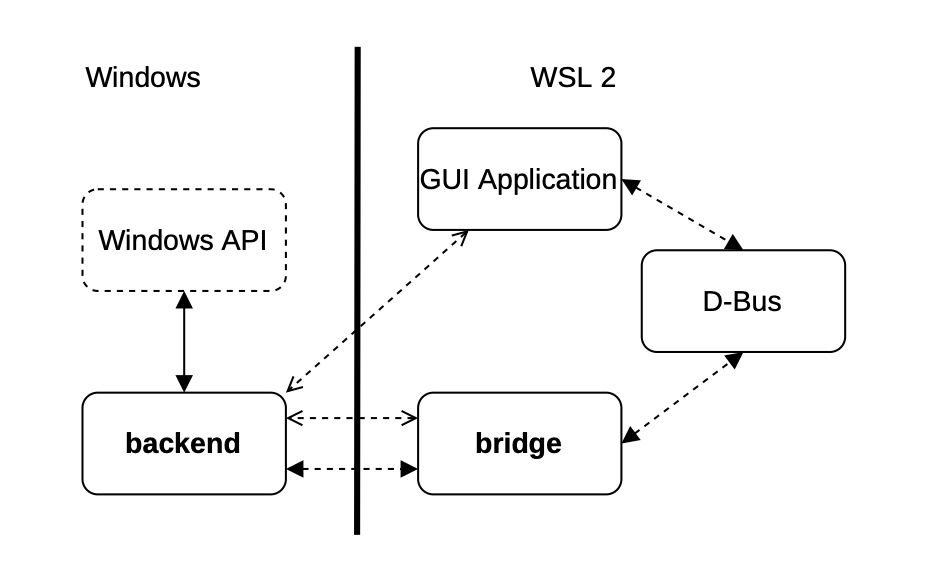
\includegraphics[width=0.75\linewidth]{assets/Screenshot 2024-01-14 at 13.31.38.png}
    \caption{Gambaran besar struktur perangkat lunak Wormhole \cite{olsen-2022-through-the-wormhole}}
    \label{olsen-wormhole-processes-basic-structure}
\end{figure}

Secara garis besar, pengimplementasian oleh Olsen (Wormhole) memiliki perbedaan dengan tugas akhir ini (FancyWSL) dalam tiga aspek:
\begin{itemize}
    \item cakupan fungsionalitas yang diintegrasikan (FancyWSL juga mengimplementasikan sistem notifikasi, serupa dengan Wormhole, tetapi dengan tambahan fungsionalitas kontrol media),
    \item metode penghubungan (\textit{bridging}) kedua lingkungan yang digunakan (FancyWSL memanfaatkan metode transportasi TCP yang tersedia pada D-Bus dengan mekanisme yang cukup berbeda dengan mekanisme yang Olsen lakukan di Wormhole), dan
    \item perlunya pengembangan perangkat lunak pengelola sesi (\textit{session manager}) D-Bus (systemd telah didukung oleh WSL sejak September 2022 \cite{systemd-support-is-now-available-in-wsl} dan telah menjadi \textit{default} pada instalasi distribusi Ubuntu di WSL sejak perilisan Ubuntu 23.04 pada April 2023 \cite{ubuntu-2304-release-roundup-systemd-now-becomes-default-for-ubuntu-on-wsl} sehingga pengelolaan sesi bus perpesanan D-Bus saat ini telah berada di bawah kontrol systemd seperti halnya pada sistem operasi Linux asli; ketiadaan pembahasan systemd oleh Olsen mengindikasikan bahwa waktu pengembangan Wormhole terjadi sebelum hadirnya dukungan systemd tersebut sehingga diperlukan pengembangan perangkat lunak \textit{session manager} tersendiri pada saat itu).
\end{itemize}

\subsection{Antarmuka Notifikasi}

Karya tulis kedua yang dibahas adalah sebuah tesis master berjudul "Notifications in a Multi-Device Environment" yang ditulis oleh Dominik Weber dan dipublikasikan pada tahun 2015 \cite{weber2015notifications}. Secara garis besar, Weber membahas penanganan notifikasi antarperangkat yang memfokuskan pada aspek pengumpulan data dari pengguna. Dalam sisi teknis, Weber membahas pengimplementasian notifikasi multiperangkat dalam bentuk ekstensi \textit{browser} Google Chrome. Karya tulis oleh Weber ini memiliki sejumlah perbedaan dengan tugas akhir ini:
\begin{itemize}
    \item Weber mengimplementasikan sistem notifikasi menggunakan ekstensi \textit{browser} Google Chrome, sedangkan tugas akhir ini mengimplementasikan sistem notifikasi dalam bentuk yang lebih \textit{native}, yakni perangkat lunak berbasis bahasa pemrograman Python.

    \item Penelitian Weber lebih berfokus ke aspek pengguna (dibuktikan dengan banyaknya survei yang dilakukan) dibandingkan dengan aspek teknis pengimplementasian; tugas akhir ini lebih berfokus pada aspek pengimplementasian dan pengujian dilakukan secara mandiri oleh diri penulis sendiri.
\end{itemize}

\subsection{Arsitektur Penjalanan Sistem}

Karya tulis ketiga yang dibahas adalah sebuah prosiding berjudul "Memory forensics and the Windows Subsystem for Linux" oleh Nathan Lewis, Andrew Case, Aisha Ali-Gombe, dan Golden G. Richard III yang dipublikasikan pada tahun 2018 \cite{lewis2018memory}. Lewis et al. utamanya membahas pembawaan dukungan berkas-berkas \textit{executable} jenis baru, \textit{executable and linkable format} (ELF), yang umumnya berada di sistem operasi Linux ke sistem operasi Windows melalui Windows Subsystem for Linux (WSL); bersamaan dengan dukungan baru ini, terdapat peningkatan \textit{attack surface} yang, misalnya, dapat diretas oleh peretas. Pada karya tulis ini, Lewis et al. membahas tentang mekanisme internal WSL, berkas-berkas \textit{executable} PE (\textit{portable executable}) dan ELF (\textit{executable and linkable format}), dan forensik memori yang dilakukan terhadap aspek-aspek tersebut sehingga cukup berbeda dengan tugas akhir ini yang membahas WSL beserta aspek-aspek integrasinya.

\section{Dasar Teori}

\subsection{Antarmuka Sistem Operasi (\textit{Shell})}

Sistem operasi tersusun atas sejumlah komponen, mulai dari komponen terdalam yang menyentuh perangkat-perangkat keras hingga komponen yang berantarmuka langsung dengan pengguna. Beberapa di antara komponen-komponen tersebut yakni \textit{kernel}, \textit{driver}, perangkat lunak sistem, \textit{shell}, dan perangkat lunak pengguna (aplikasi). Salah satu komponen yang krusial ialah \textit{shell} yang bertugas memberikan antarmuka bagi pengguna untuk dapat berinteraksi dengan sistem operasi tersebut.

Penggunaan istilah "\textit{shell}" untuk menandakan antarmuka sistem operasi pertama kali terjadi pada sekitar tahun 1964--1965 oleh Louis Pouzin ketika sedang mengembangkan sistem operasi Multics \cite{origin-of-the-shell-name}. Istilah \textit{shell} digunakan karena komponen ini adalah bagian sistem operasi terluar yang berinteraksi secara langsung dengan dunia luar dan mengelilingi komponen-komponen sistem operasi di bawahnya, sehingga dapat dianalogikan sebagai "cangkang" dari sistem operasi \cite{shell-jargon-explanation}.

Secara umum, terdapat berbagai jenis \textit{shell} yang digunakan oleh sistem-sistem operasi modern saat ini:
\begin{itemize}
    \item \textbf{\textit{Shell} berantarmuka grafis (\textit{graphical user interface})}\\
    \textit{Shell} jenis ini merupakan \textit{shell} yang paling sering pengguna temui pada zaman modern ini. Sebagian besar pengguna saat ini berinteraksi dengan perangkat komputer mereka melalui metode interaksi grafis. Antarmuka tempat pengguna berinteraksi tersebut sesungguhnya merupakan komponen \textit{shell} yang merupakan bagian dari sistem operasi pada perangkat yang bersangkutan. Sebagai contoh, \textit{shell} grafis pada sistem operasi Windows 11 terdiri atas \textit{taskbar} yang terletak di bawah layar, menu Start yang dapat dimunculkan dengan menekan tombol Start (tombol berlogo Windows di dalam \textit{taskbar}), pusat pemberitahuan/notifikasi, dan bilah pengaturan cepat (\textit{quick settings}).
    
    \item \textbf{\textit{Shell} berantarmuka baris perintah (\textit{command-line interface})}\\
    \textit{Shell} jenis ini telah ada terlebih dahulu sebelum dikembangkannya \textit{shell} berantarmuka grafis. Pada zaman modern ini, \textit{shell} berantarmuka baris perintah pun masih sering digunakan, terutama untuk kegunaan pengaksesan fungsionalitas sistem operasi tingkat lanjut, administrasi sistem, dan otomasi (\textit{scripting}). Beberapa contoh \textit{shell} berantarmuka baris perintah modern yakni PowerShell di sistem operasi Windows serta Bourne shell (\verb|sh|), Bourne-Again Shell (\verb|bash|), Z shell (\verb|zsh|), KornShell (\verb|ksh|), dan Fish shell (\verb|fish|) di sistem operasi Linux \cite{kidwai2021comparative}.
\end{itemize}

\subsection{Linux, "Mirip Unix", dan Standar POSIX}

Linux merupakan keluarga sistem operasi

\subsection{D-Bus}

D-Bus merupakan sistem komunikasi antarproses (\textit{interprocess communication}) yang populer digunakan di sebagian besar distribusi Linux. Sesuai dengan namanya, D-Bus bekerja dengan konsep arsitektur "bus" yang berarti terdapat sebuah kanal utama (bus) sebagai jalur pertukaran informasi dan terdapat sejumlah klien yang terhubung dengan kanal utama (bus) tersebut. Secara garis besar, terdapat dua komponen utama dalam penggunaan sistem D-Bus:

\begin{itemize}
    \item \textbf{\textit{Server} atau \textit{daemon} D-Bus}\\
    \textit{Server} D-Bus bertindak sebagai penyedia bus sentral tempat klien-klien D-Bus terhubung. \textit{Server} D-Bus bertugas mengelola klien-klien yang terhubung dan menyalurkan data dari sumbernya ke tujuannya dengan benar \cite{qt-introduction-to-dbus}. \textit{Server} D-Bus umumnya dijalankan oleh sebuah proses yang bernama \textit{daemon} D-Bus yang umumnya memiliki nama berkas \textit{executable} "\path{dbus-daemon}".

    \item \textbf{Klien D-Bus}\\
    Klien D-Bus merupakan istilah untuk tiap-tiap perangkat lunak yang terhubung ke bus utama D-Bus. Klien D-Bus dapat bertindak sebagai penyedia layanan (\textit{provider}) ataupun sebagai aplikasi reguler yang mengonsumsi layanan (\textit{consumer}).
\end{itemize}

\begin{figure}
    \centering
    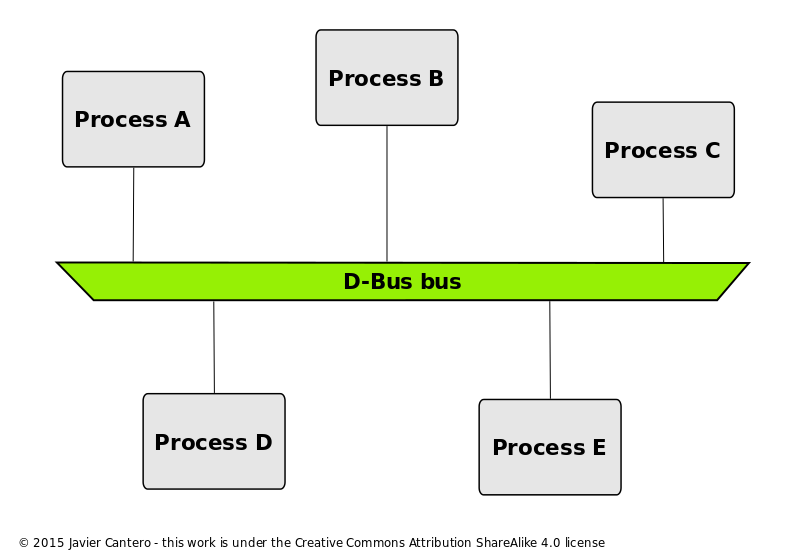
\includegraphics[width=0.75\linewidth]{assets/dbus-analogy-diagram.png}
    \caption{Ilustrasi bus perpesanan D-Bus \cite{dbus-bus-illustration}}
    \label{fig:enter-label}
\end{figure}

\begin{figure}
    \centering
    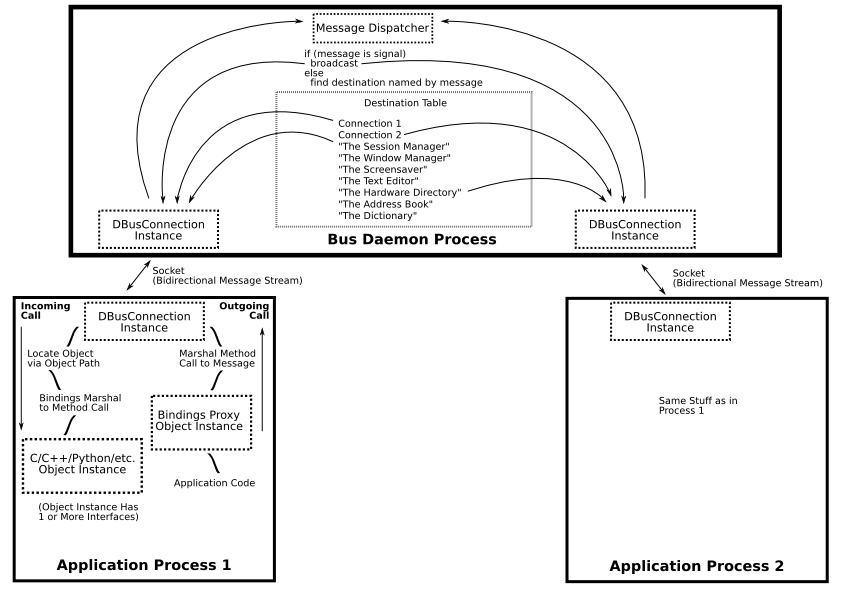
\includegraphics[width=1\linewidth]{assets/dbus-diagram.png}
    \caption{Diagram mendetail arsitektur D-Bus \cite{dbus-main-project-page}}
    \label{fig:enter-label}
\end{figure}

Dalam suatu sistem operasi yang sedang berjalan, dimungkinkan penjalanan lebih dari satu bus dalam satu waktu. Pada sistem operasi Linux, umumnya digunakan dua buah bus yang memiliki peran masing-masing, yaitu bus sistem (\textit{system bus}) dan bus sesi (\textit{session bus}). Bus sistem digunakan untuk mengelola dan mengadministrasi hal-hal yang bersifat penting terhadap berjalannya sistem operasi, seperti penyambungan perangkat keras baru, peringatan baterai lemah, dan status jaringan \cite{will2020trusted}. Bus sistem berjalan secara \textit{system-wide} sehingga mencakup seluruh sesi pengguna yang sedang berjalan di sistem operasi. Di sisi lain, bus sesi digunakan untuk hal-hal yang bersifat lebih mengarah ke pengguna (\textit{user-facing}) seperti pengiriman notifikasi dan sistem kontrol media, dua hal yang menjadi topik utama tugas akhir ini. Bus sesi tersedia secara lokal di tiap-tiap sesi pengguna yang sedang berjalan di suatu sistem operasi. Istilah "bus perpesanan D-Bus", "\textit{server} D-Bus", dan "\textit{daemon} D-Bus" dapat dikatakan identik dalam konteks ini; tiap-tiap bus memiliki \textit{instance} \textit{daemon} D-Bus-nya masing-masing, sehingga sistem operasi Linux secara \textit{default} memiliki dua buah \textit{instance} \textit{daemon} D-Bus yang berjalan dalam satu waktu.

Agar dapat dihubungi oleh para klien, tiap-tiap bus perpesanan D-Bus memiliki alamat yang diatur pada awal penjalanan \textit{daemon} D-Bus. Bentuk alamat yang digunakan oleh bus perpesanan D-Bus berbeda-beda sesuai dengan metode transportasi yang digunakan. Berdasarkan spesifikasi D-Bus \cite{dbus-specification}, terdapat sejumlah metode transportasi yang didukung oleh D-Bus:
\begin{itemize}
    \item \textbf{Soket Unix}\\
    Metode transportasi berbasis soket Unix menggunakan berkas soket Unix yang terletak secara lokal pada \textit{file system}. Metode transportasi ini hanya didukung apabila \textit{daemon} D-Bus berjalan di sistem operasi berbasis Unix atau mirip Unix seperti Linux dan macOS. Metode transportasi ini digunakan apabila penulisan alamat diawali oleh "\verb|unix:|".

    \item \textbf{systemd}\\
    Metode transportasi berbasis systemd memiliki konsep serupa dengan metode transportasi berbasis soket Unix, tetapi memanfaatkan sistem pengelolaan soket otomatis bernama aktivasi soket (\textit{socket activation}) yang dilakukan oleh systemd. Metode transportasi ini memanfaatkan informasi soket yang dikelola oleh systemd untuk digunakan sebagai metode transportasi D-Bus. Seperti namanya, metode transportasi ini hanya tersedia pada sistem operasi Linux yang menggunakan systemd sebagai sistem init-nya. Metode transportasi ini digunakan apabila penulisan alamat berisikan "\verb|systemd:|".
    
    \item \textbf{launchd}\\
    Metode transportasi berbasis launchd juga memiliki konsep yang serupa dengan metode transportasi berbasis soket Unix, tetapi memanfaatkan soket Unix yang telah dialokasikan oleh launchd. Mengingat sistem init launchd hanya tersedia pada sistem operasi macOS, metode transportasi ini hanya didukung apabila \textit{daemon} D-Bus berjalan di sistem operasi macOS. Metode transportasi ini digunakan apabila penulisan alamat berisikan "\verb|launchd:|".
    
    \item \textbf{TCP}\\
    Metode transportasi berbasis TCP memanfaatkan protokol TCP (Transmission Control Protocol) sebagai metode komunikasi antarklien D-Bus, baik yang terletak pada perangkat komputer yang sama maupun yang terletak pada perangkat komputer yang berbeda (\textit{remote}). Metode transportasi ini merupakan satu-satunya metode transportasi yang tersedia apabila \textit{daemon} D-Bus berjalan pada sistem operasi Windows mengingat metode-metode transportasi yang lain tidak didukung pada sistem operasi Windows. Metode transportasi ini digunakan apabila penulisan alamat diawali oleh "\verb|tcp:|" dan diikuti oleh properti-properti yang terdiri dari "\verb|host|" (wajib), "\verb|bind|" (opsional), "\verb|port|" (opsional), dan "\verb|family|" (opsional) yang penulisannya dipisahkan oleh tanda koma (misalnya "\path{tcp:localhost,port=12345,family=ipv4}").

    \item \textbf{TCP dengan metode otentikasi nonce}\\
    Metode transportasi ini identik dengan metode transportasi berbasis TCP biasa, tetapi dengan tambahan lapisan keamanan berupa otentikasi berbasis nonce. Metode otentikasi berbasis nonce memastikan bahwa hanya klien yang memiliki akses baca (\textit{read access}) pada suatu lokasi tertentu di \textit{file system} dapat terhubung ke \textit{server} D-Bus. Metode transportasi ini memiliki format penulisan alamat yang serupa dengan metode transportasi berbasis TCP biasa (sama-sama berawalan "\verb|tcp:|" dengan tambahan properti "\verb|noncefile|".

    \item \textbf{Subproses}\\
    Metode transportasi berbasis subproses bekerja dengan cara melakukan \textit{fork} pada suatu proses dan menghubungkan \textit{standard input} dan \textit{standard output} proses tersebut ke sebuah soket Unix anonim. Metode transportasi ini tidak tersedia pada sistem operasi Windows. Metode transportasi ini digunakan apabila alamat diawali oleh "\verb|unixexec:|".
\end{itemize}

Seperti yang telah disebutkan pada tiap-tiap deskripsi metode transportasi di atas, metode transportasi ditentukan secara otomatis sesuai dengan format penulisan alamat bus perpesanan D-Bus yang telah diatur. Alamat bus perpesanan D-Bus dapat diatur melalui dua tempat: argumen penjalanan \textit{daemon} D-Bus dan berkas konfigurasi. Metode pengaturan alamat bus perpesanan D-Bus melalui argumen penjalanan \textit{daemon} D-Bus dilakukan dengan menambahkan argumen berbentuk \lstinline[language=bash,columns=fixed]{--address="<tuliskan alamat yang diinginkan di sini>"}. Metode pengaturan alamat melalui argumen akan menimpa (\textit{override}) pengaturan apa pun yang dilakukan di berkas konfigurasi. Di sisi lain, metode pengaturan alamat bus perpesanan D-Bus melalui berkas konfigurasi dilakukan dengan cara memodifikasi berkas konfigurasi \textit{default} yang telah ada (berkas konfigurasi \textit{default} bus sistem berada di \path{/usr/share/dbus-1/system.conf} dan berkas konfigurasi \textit{default} bus sesi berada di \path{/usr/share/dbus-1/session.conf}) atau membuat berkas konfigurasi baru berekstensi berkas "\verb|.conf|" dan memuatnya pada saat penjalanan \textit{daemon} D-Bus melalui argumen \lstinline[language=bash,columns=fixed]{--config-file=<lokasi berkas konfigurasi>}.

Dalam mengidentifikasi dirinya sendiri dan berkomunikasi dengan klien lain, tiap-tiap klien yang terhubung dengan bus perpesanan D-Bus mengemban sejumlah elemen yang didesain agar memiliki kemiripan dengan konsep-konsep pemrograman berorientasi objek yang telah familier bagi banyak orang. Berikut elemen-elemen yang dimaksud.
\begin{itemize}
    \item \textbf{Nama bus (\textit{bus name})}\\
    Tiap-tiap klien D-Bus memiliki identitas berupa "nama bus" yang digunakan untuk mengidentifikasi klien tersebut dalam suatu bus perpesanan D-Bus. Nama bus terdiri dari dua jenis, nama bus unik (\textit{unique name}) dan nama bus yang dikenal (\textit{well-known name}), dan tiap-tiap klien dapat memiliki lebih dari satu nama bus. Secara \textit{default}, tiap-tiap klien baru yang terhubung ke suatu bus perpesanan D-Bus akan mendapatkan nama bus unik (diberikan secara otomatis oleh \textit{daemon} D-Bus) yang tersusun atas sejumlah angka yang dimulai oleh tanda titik dua (misalnya ":34.907"). Perlu diingat bahwa istilah "nama bus" di sini berarti nama masing-masing klien yang terhubung dalam suatu bus perpesanan, bukan nama bus perpesanan itu sendiri \cite{official-introduction-to-dbus}.
    \item \textbf{Objek (\textit{object})}\\
    Objek dalam konteks komunikasi D-Bus merupakan ujung-ujung komunikasi (\textit{endpoint}) yang dimiliki oleh klien di dalam suatu bus perpesanan D-Bus. Tiap-tiap klien D-Bus dapat memiliki lebih dari satu objek.
    \item \textbf{Antarmuka (\textit{interface})}\\
    Antarmuka dalam konteks komunikasi D-Bus merupakan suatu "kontrak" yang disetujui oleh berbagai klien yang digunakan untuk memfasilitasi komunikasi antarklien. Antarmuka diperlukan agar dua klien dapat berkomunikasi dengan bentuk dan struktur data yang sama yang telah disetujui oleh masing-masing pihak.
\end{itemize}

Secara garis besar, proses komunikasi di dalam suatu bus perpesanan D-Bus dilakukan dalam bentuk "pesan" (\textit{message}). Pesan-pesan dalam D-Bus dapat dikategorikan menjadi dua jenis di bawah ini yang juga memiliki kemiripan dengan konsep pemrograman berorientasi objek.
\begin{itemize}
    \item \textbf{Metode (\textit{method})}\\
    Metode merupakan pesan yang dikirimkan secara spesifik dan terarah dari klien pengirim (\textit{sender}) ke tujuan (\textit{destination}) yang jelas. Pesan jenis metode dikirimkan dengan cara memanggil metode yang bersangkutan pada objek D-Bus yang diinginkan.
    \item \textbf{Sinyal (\textit{signal})}\\
    Sinyal merupakan pesan yang dikirimkan secara tidak terarah (tidak memiliki tujuan spesifik). Pesan berjenis sinyal disebarluaskan (\textit{advertise}) di dalam bus perpesanan untuk didengarkan oleh klien-klien lain yang berkepentingan.
\end{itemize}

Selain dua jenis pesan di atas, objek-objek pada klien D-Bus juga memiliki elemen bernama "properti" (\textit{property}) yang juga berkonsep serupa dengan pemrograman berorientasi objek. Properti pada suatu objek D-Bus umumnya berisi informasi-informasi yang berkaitan dengan objek tersebut dan/atau klien yang memiliki objek tersebut. Pada umumnya, setiap pergantian nilai properti akan menyebabkan sinyal bernama "PropertiesChanged" pada antarmuka "org.freedesktop.DBus.Properties" tersebar sehingga pergantian nilai properti tersebut dapat diketahui oleh klien-klien lain yang berkepentingan.

Dalam menginspeksi bus perpesanan D-Bus, terdapat berbagai macam perangkat lunak atau peralatan (\textit{tools}) yang dapat membantu. Secara \textit{default}, perangkat lunak D-Bus yang terinstal juga memiliki peralatan-peralatan bawaan seperti \verb|dbus-monitor| dan \verb|dbus-send| yang dapat bermanfaat untuk memeriksa serta berinteraksi langsung dengan bus perpesanan D-Bus dalam antarmuka baris perintah (\textit{command-line interface}). Selain itu, tersedia pula solusi-solusi pihak ketiga seperti perangkat lunak D-Feet yang dapat memeriksa bus perpesanan D-Bus dalam antarmuka grafis (\textit{graphical user interface}).

\begin{figure}[h]
    \centering
    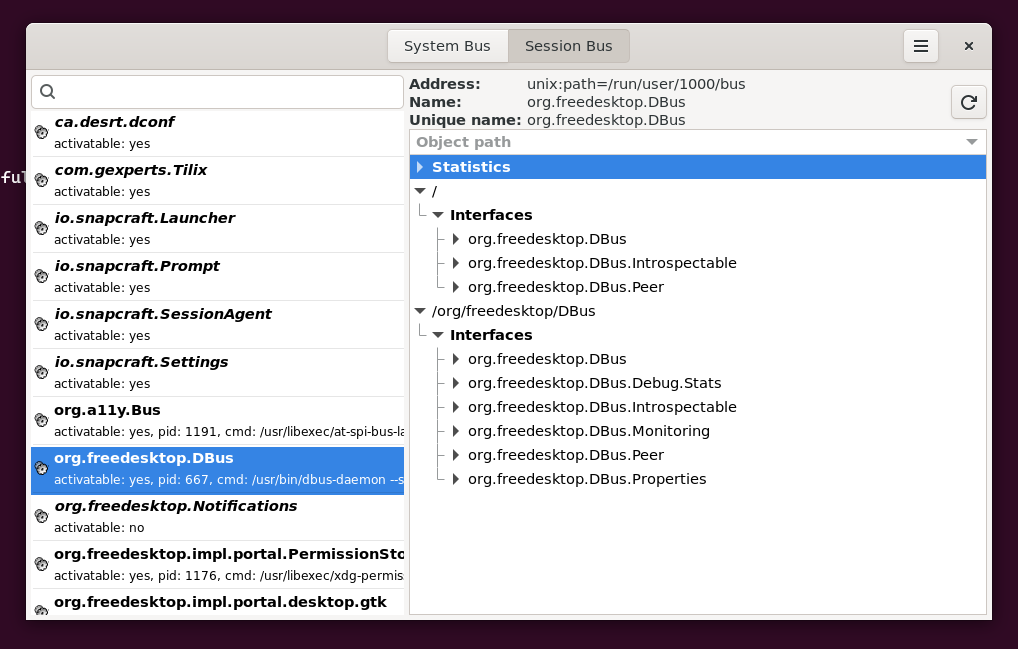
\includegraphics[width=0.75\linewidth]{assets/dfeet-window-screenshot.png}
    \caption{Tangkapan layar perangkat lunak "D-Feet" yang berjalan di Windows Subsystem for Linux (WSL)}
    \label{fig:enter-label}
\end{figure}

% \subsection{Sistem Init systemd}

% systemd merupakan salah satu sistem init yang tersedia untuk digunakan di sistem operasi Linux di samping sistem-sistem init lain seperti SysV Init, .

\subsection{Windows Subsystem for Linux (WSL)}

Windows Subsystem for Linux merupakan usaha Microsoft dalam membawa kompatibilitas Unix/Linux ke dalam lingkungan Windows. Secara garis besar, terdapat dua versi WSL yang telah dirilis dengan konsep dan arsitektur yang berbeda.
\begin{itemize}
    \item \textbf{Windows Subsystem for Linux versi 1 (WSL1)}
    WSL1 memanfaatkan sebuah lapisan penerjemah panggilan-panggilan sistem (\textit{syscalls}) yang dipanggil oleh perangkat-perangkat lunak Linux agar diterjemahkan menjadi panggilan-pangiglan sistem (\textit{syscalls}) ekuivalen yang terdapat di Windows. WSL1 adalah varian WSL yang diluncurkan pada pengenalan WSL pertama kali di Windows 10 pada tahun 2016.

    \item \textbf{Windows Subsystem for Linux versi 2 (WSL2)}
    WSL2 memanfaatkan sebuah \textit{virtual machine} Hyper-V dengan sejumlah integrasi lebih lanjut agar tidak terasa seperti penjalanan \textit{virtual machine} tradisional. WSL2 menjalankan \textit{kernel} Linux asli yang tervirtualisasi sehingga meningkatkan cakupan dukungan perangkat lunak Linux dibandingkan dengan WSL1.
\end{itemize}

% Pada perheletan pengembang tahunan Microsoft Build 2021, Microsoft menyatakan bahwa mereka akan mendukung 

Pada tahun 2021, Microsoft merilis sistem operasi Windows 11 yang membawa sejumlah perkembangan; salah satu perkembangan tersebut terdapat pada WSL. Windows 11 mendukung penjalanan perangkat lunak Linux berantarmuka grafis (GUI) secara langsung. Microsoft menamakan fitur baru ini "Windows Subsystem for Linux GUI (WSLg)".

\begin{figure}
    \centering
    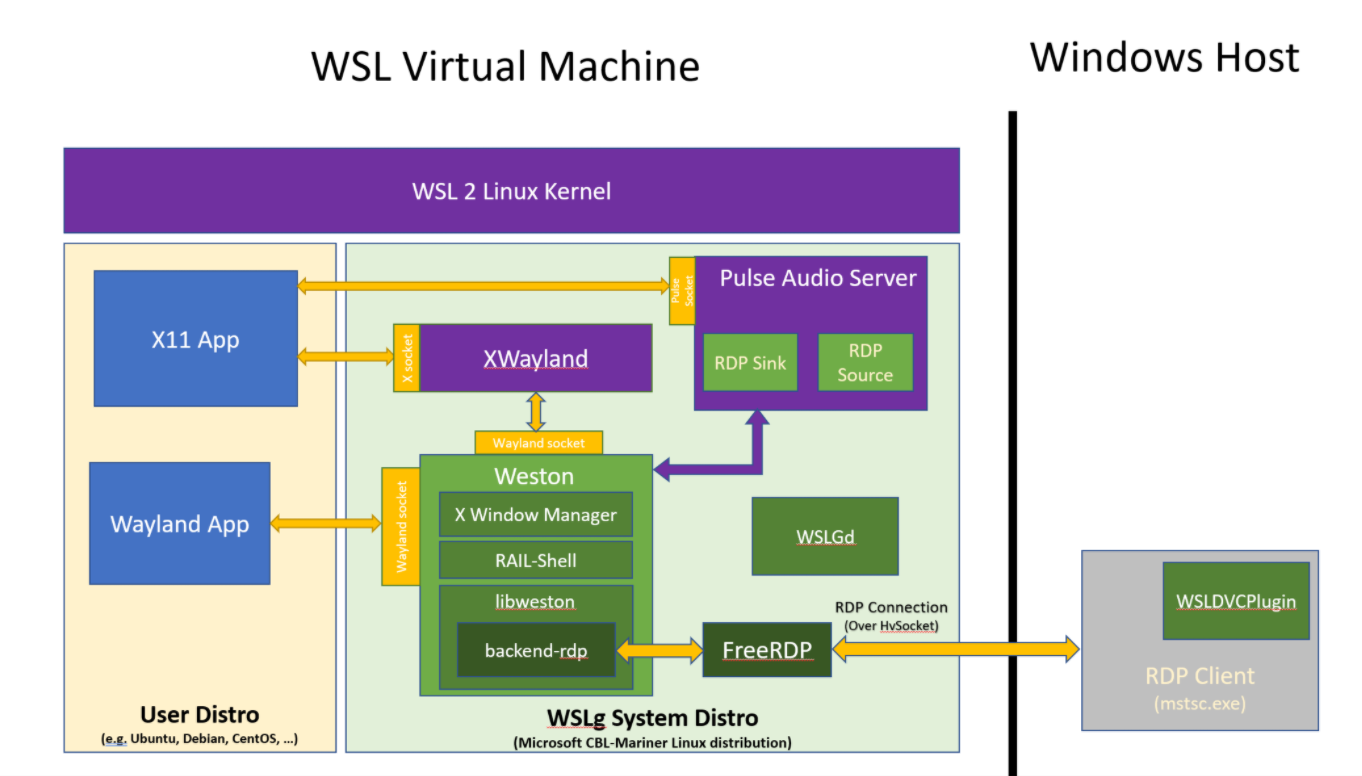
\includegraphics[width=1\linewidth]{assets/wslg-architecture.png}
    \caption{Arsitektur Windows Subsystem for Linux GUI (WSLg) \cite{wslg-architecture}}
\end{figure}

% https://link.springer.com/chapter/10.1007/978-1-4842-6873-5_1

\section{Analisis Perbandingan Metode}

Dalam penyusunan tugas akhir ini, penulis mengkaji serta membandingkan metode-metode yang mungkin dilakukan untuk sejumlah aspek pengerjaan. Aspek-aspek yang dimaksud yaitu penghubungan (\textit{bridging}) lingkungan Windows Subsystem for Linux (WSL) dengan lingkungan \textit{host} Windows dan penentuan bahasa dan platform pemrograman yang paling praktis dan cocok digunakan dalam pengembangan perangkat lunak yang terlibat.

\subsection{Penghubungan Lingkungan Windows Subsystem for Linux (WSL) dengan Lingkungan \textit{Host} Windows}

Dalam aspek penghubungan lingkungan Windows Subsystem for Linux (WSL) dengan lingkungan \textit{host} Windows, metode yang dipilih menentukan jumlah dan cakupan perangkat lunak yang perlu dikembangkan, tingkat kesulitan pengembangan perangkat lunak tersebut, serta efisiensi penjalanan perangkat lunak yang telah jadi. Berikut pemaparan empat metode yang mungkin dilakukan.
\begin{enumerate}
    \item Lingkungan WSL dihubungkan dengan lingkungan \textit{host} Windows melalui \textit{socket} Unix. Hal ini dimungkinkan dengan diperkenalkannya dukungan \textit{socket} Unix (AF\_UNIX) pada sistem operasi Windows 10 ke atas pada tahun 2017 \cite{bringing-afunix-to-windows}. Namun, penelusuran lebih lanjut mengindikasikan bahwa kemampuan ini rupanya hanya mendukung Windows Subsystem for Linux versi 1 (WSL1) dan belum mendukung Windows Subsystem for Linux versi 2 (WSL2) \cite{github-issues-afunix-not-supported-in-wsl2}. Oleh karena itu, mengingat kemampuan grafis (\textit{graphical user interface}) pada Windows Subsystem for Linux hanya tersedia pada Windows Subsytem for Linux versi 2 (WSL2), metode ini tidak relevan dengan tujuan skripsi ini.
    
    \item Lingkungan WSL dihubungkan dengan lingkungan \textit{host} Windows dengan memanfaatkan \textit{server} HTTP. Metode ini ikut dipertimbangkan mengingat pengalaman penulis yang cukup banyak berhubungan dengan bidang pengembangan web (\textit{web development}). Metode ini dapat dibagi kembali menjadi dua submetode:
    
    \begin{enumerate}
        \item Penghubungan kedua lingkungan melibatkan dua buah \textit{server} HTTP yang masing-masing berjalan di sisi WSL dan di sisi \textit{host} Windows. Dua buah \textit{server} diperlukan karena komunikasi bersifat dua arah: WSL mengirimkan konten yang ingin ditampilkan ke sisi \textit{host} Windows dan \textit{host} Windows mengomunikasikan hasil interaksi pengguna (\textit{user input}) kembali ke sisi WSL. Meskipun implementasi submetode ini dapat dibuat seefisien mungkin, penjalanan dua buah \textit{server} tetap saja terasa kurang efisien, terutama bila dibandingkan dengan metode-metode lainnya.
        
        \item Penghubungan kedua lingkungan menggunakan cukup satu buah \textit{server} saja untuk menghindari duplikasi penggunaan \textit{resources}, tetapi memanfaatkan teknologi yang memungkinkan komunikasi secara dua arah seperti HTTP \textit{long polling} dan WebSocket. Penggunaan HTTP \textit{long polling} memiliki kemungkinan menghasilkan performa yang kurang efisien \cite{problems-in-http-long-polling}, sedangkan penggunaan WebSocket sama saja dengan penggunaan Unix \textit{socket} biasa namun dengan \textit{overhead} protokol HTTP yang dapat berefek pada performa.
    \end{enumerate}
    
    \item Lingkungan WSL dihubungkan dengan lingkungan \textit{host} Windows dengan komunikasi secara tekstual atau terserialisasi (\textit{serialized}). Pertukaran informasi berbentuk teks (tekstual) ini dapat melalui berbagai perantara; berikut beberapa di antaranya.
    \begin{enumerate}
        \item Informasi tekstual dipertukarkan melalui berkas \textit{executable} pembantu (\textit{helper}) sebagai argumen pengeksekusian berkas \textit{executable} tersebut. Ditentukan dua buah berkas \textit{executable} yang masing-masing bertugas mengirimkan informasi ke sisi \textit{host} Windows dan mengirimkan informasi ke sisi WSL. Pada sisi WSL, hal ini dimungkinkan oleh kemampuan WSL menjalankan berkas \textit{executable} Windows (umumnya berekstensi \verb|.exe|) secara langsung di dalam \textit{command-line} WSL \cite{msdocs-run-windows-tools-from-linux}. Pada sisi Windows, hal ini dimungkinkan oleh kemampuan memanggil WSL secara programatik atau \textit{scripted} dengan perintah yang telah ditetapkan. Sebagai contoh, pengiriman informasi dari sisi WSL dapat dilakukan dengan perintah
        \begin{lstlisting}[language=bash]
# Di shell bash
/path/to/fwsl-send-to-windows.exe --data="<insert JSON-serialized data here>"\end{lstlisting}
        dan pengiriman informasi dari sisi Windows ke sisi WSL dapat dilakukan dengan perintah
        \begin{lstlisting}
# Di shell PowerShell atau cmd.exe
wsl.exe /path/to/fwsl-send-to-wsl --data="<insert JSON-serialized data here>"\end{lstlisting}

        \item Informasi tekstual dipertukarkan melalui mekanisme \textit{piping}. Cara pertukaran data ini serupa dengan penggunaan berkas \textit{executable} pembantu (\textit{helper}) pada submetode (a), namun data disalurkan melalui \textit{standard stream} (seperti \textit{standard input} dan \textit{standard output}) dan dihubungkan dengan \textit{pipe} alih-alih diletakkan sebagai argumen suatu berkas \textit{executable}. Pertukaran data dengan cara ini tetap memerlukan berkas-berkas \textit{executable} sebagai pengirim dan/atau penerima data. Tetapi, berbeda dengan submetode (a), submetode ini memungkinkan penggunaan perangkat lunak utama itu sendiri sebagai pengirim dan penerima data. Pertukaran data difasilitasi oleh berkas \textit{named pipe} sebanyak dua buah yang masing-masing menangani pengiriman data ke tiap-tiap arah (menuju Windows dan menuju WSL).
        \begin{verbatim}
 ________________               ________________
|                |             |                |
|           StdIn(== ← === ← ==(StdOut          |
|    Windows     |             |   WSL bridge   |
|    bridge      |             |                |
|          StdOut)== → === → ==)StdIn           |
|________________|             |________________|

        \end{verbatim}

        \item Informasi tekstual dipertukarkan dengan memanfaatkan perintah \verb|dbus-send| dan \verb|dbus-monitor| secara programatik. Mengingat topik utama skripsi ini selalu berkaitan dengan protokol D-Bus, submetode ini dapat mensimplifikasi rangkaian proses pengerjaan karena menggunakan peralatan yang berasal dari D-Bus itu sendiri. Sebagai contoh, dengan pemantauan keluaran (\textit{output}) perintah \verb|dbus-monitor|, pemulaian pemutaran media (musik, video, dan lain-lain) dari suatu perangkat lunak yang berjalan di dalam WSL menghasilkan keluaran
        \begin{lstlisting}
signal time=1702386858.242218 sender=:1.19 -> destination=(null destination) serial=24 path=/org/mpris/MediaPlayer2; interface=org.freedesktop.DBus.Properties; member=PropertiesChanged
   string "org.mpris.MediaPlayer2.Player"
   array [
      dict entry(
         string "PlaybackStatus"
         variant             string "Playing"
      )
   ]
   array [
   ]\end{lstlisting}
        dan apabila pemutaran media tersebut ingin dijeda (\textit{pause}), dapat dijalankan perintah berikut
        \begin{lstlisting}[language=bash]
dbus-send --dest=org.mpris.MediaPlayer2.spotify /org/mpris/MediaPlayer2 org.mpris.MediaPlayer2.Player.PlayPause\end{lstlisting}
        Meskipun demikian, proses integrasi dalam skripsi ini melibatkan lebih dari sekadar perintah-perintah D-Bus dan dapat dipastikan membutuhkan perangkat lunak tambahan. Sebagai contoh, sejumlah fungsi yang dilayani melalui D-Bus seperti penanganan notifikasi memerlukan layanan (\textit{service}) yang diregistrasikan secara eksplisit di bus perpesanan D-Bus yang bersangkutan; submetode ini hanya mengandalkan metode yang serupa dengan "\textit{sniffing}" dan tidak benar-benar memiliki identitas dan keberadaan yang teregistrasi sehingga fungsi penanganan notifikasi tetap tidak akan bisa bekerja. Oleh karena itu, akan lebih baik apabila seluruh fungsionalitas dan logika dalam pengerjaan skripsi ini disatukan ke dalam perangkat lunak tambahan tersebut. Selain itu, keluaran (\textit{output}) perintah \verb|dbus-monitor| tidak selalu lengkap (pada contoh keluaran perintah \verb|dbus-monitor| di atas, tidak ada informasi bahwa perangkat lunak Spotify adalah perangkat lunak yang memulai memainkan media), sehingga submetode ini kurang bisa diandalkan.
    \end{enumerate}
    
    \item Lingkungan Windows Subsystem for Linux (WSL) dihubungkan dengan lingkungan \textit{host} Windows dengan meng-\textit{extend} jangkauan bus perpesanan D-Bus hingga dapat diakses secara langsung di dalam lingkungan Windows, sehingga perangkat lunak di Windows dapat langsung menghubungi bus perpesanan D-Bus yang berjalan di WSL. Hal ini dicapai dengan cara mengatur konfigurasi \verb|dbus-daemon| di WSL agar dapat diakses melalui TCP (di samping konfigurasi soket Unix \textit{default} yang telah ada) dan mengonsumsi alamat TCP yang ditentukan di perangkat lunak \textit{bridge} yang berjalan di Windows. Metode ini memiliki keuntungan tersendiri: mengingat koneksi bus perpesanan D-Bus saat ini tersedia secara langsung di lingkungan Windows, penyediaan \textit{notification server} dan \textit{MPRIS server} dapat dilakukan secara langsung oleh perangkat lunak \textit{bridge} di sisi Windows, sehingga menghilangkan kebutuhan penjalanan perangkat lunak \textit{bridge} kedua di lingkungan WSL.
\end{enumerate}

Bila disimpulkan kembali, perbandingan keempat metode di atas dapat dilihat pada \autoref{} berikut.

\begin{table}
    \centering
    \caption{Perbandingan metode penghubungan dengan bus perpesanan D-Bus di WSL}
    \label{perbandingan-metode-penghubungan-dengan-dbus-di-wsl}
    \begin{tabularx}{\textwidth}{|l|X|X|X|X|} \hline
        \textbf{No.} & \textbf{Metode} & \textbf{Kebutuhan} & \textbf{Kelebihan} & \textbf{Kekurangan}\\ \hline
        1 & Soket Unix & & Sangat efisien karena hanya melibatkan soket lokal tanpa beban \textit{overhead} tambahan & Tidak tersedia untuk WSL2 yang merupakan syarat utama WSLg\\ \hline
    \end{tabularx}
\end{table}


Berdasarkan penjabaran dan analisis perbandingan metode penghubungan lingkungan WSL dengan lingkungan \textit{host} Windows, dipilih metode keempat mengingat metode penghubungannya yang cukup \textit{straightforward} dan penggunaan protokol TCP yang relatif lebih efisien dibandingkan dengan metode-metode lainnya.

\subsection{Bahasa dan Platform Pemrograman yang Digunakan}

Dalam aspek bahasa dan platform pemrograman, dipertimbangkan berbagai hal seperti kelengkapan integrasi dengan \textit{application programming interface} (API) \textit{shell} Windows dan kemampuan berkomunikasi dengan D-Bus (baik dengan solusi bawaan atau pihak pertama, apabila tersedia, maupun dengan bantuan pustaka pihak ketiga yang tersedia pada bahasa pemrograman tersebut). Berikut perbandingan platform dan bahasa pemrograman yang dapat digunakan yang disajikan dalam bentuk tabel.

\begin{table}[h]
    \centering
    \caption{Perbandingan platform dan bahasa pemrograman.}
    \begin{tabularx}{\textwidth}{|l|X|X|} \hline
        \textbf{Platform} & \textbf{Integrasi \textit{Shell} Windows} & \textbf{Integrasi D-Bus}\\ \hline
        C\# & Tersedia (mengingat C\# adalah salah satu platform \textit{native} di Windows & Terbatas dan kurang terdokumentasi (\textit{undocumented})\\ \hline
        Python & Tersedia melalui \textit{binding} pihak ketiga & Tersedia pustaka-pustaka (\textit{library}) yang beraneka ragam\\ \hline
    \end{tabularx}
\end{table}

Meskipun bahasa pemrograman C\# didukung secara lebih baik oleh sistem operasi Windows, ketiadaan dukungan integrasi dengan D-Bus yang memungkinkan menghalangi penggunaan bahasa pemrograman C\# sebagai opsi yang \textit{viable}. Oleh karena itu, dipilih bahasa penggunaan Python yang memiliki dukungan lebih baik dalam penghubungan dengan D-Bus meskipun harus menggunakan \textit{binding} tambahan untuk mengakses beragam API yang terdapat di Windows.

\section{Pertanyaan Tugas Akhir}

Dalam serangkaian pengerjaan tugas akhir ini, penulis menemukan satu buah pertanyaan krusial yang berkaitan dengan metode yang telah dipilih. Pertanyaan-pertanyaan ini perlu dipelajari dan dijawab terlebih dahulu sebelum dapat melanjutkan ke langkah selanjutnya dalam pengerjaan.

\begin{enumerate}
    \item Perangkat lunak \verb|dbus-daemon| dapat melakukan \textit{listening} ke lebih dari satu alamat apabila telah diatur pada berkas konfigurasi (misalnya pada berkas \path{/usr/share/dbus-1/session.conf} untuk bus \textit{session}). Namun, \verb|dbus-daemon| juga memiliki seperangkat argumen eksekusi \cite{dbus-daemon-man-page} yang beberapa di antaranya dapat menimpa (\textit{override}) konfigurasi yang telah dilakukan pada berkas konfigurasi; salah satu argumen yang menarik perhatian yaitu argumen \verb|--address|. Apakah argumen ini mendukung pemberian lebih dari satu alamat? Apabila argumen ini hanya mendukung satu alamat, apa yang terjadi jika argumen ini digunakan dalam pemanggilan \verb|dbus-daemon| saat konfigurasi yang tertimpa (\textit{override}) pada berkas konfigurasi memuat lebih dari satu alamat? Apakah penggunaan argumen ini hanya menimpa (\textit{override}) satu buah alamat pada berkas konfigurasi saja atau menimpa (\textit{override}) semua alamat yang telah diatur pada berkas konfigurasi?
\end{enumerate}

\chapter{Metode Penelitian}

\section{Alat dan Bahan Tugas Akhir}

\subsection{Alat Tugas Akhir}

\begin{enumerate}
    \item Perangkat komputer, baik \textit{desktop} maupun komputer jinjing (\textit{laptop}), sebagai \textbf{komputer utama} dengan
    \begin{itemize}
        \item sistem operasi Windows 11 Home, Pro, atau SKU lain yang mendukung kapabilitas Windows Subsystem for Linux versi 2 (WSL2);
        \item arsitektur x86\_64 (64-bit) dengan prosesor seri Intel Core generasi ke-8 atau lebih tinggi;
        \item memori (RAM) minimal 8 GB; dan
        \item ruang penyimpanan minimal 64 GB.
    \end{itemize} Bila menggunakan \textit{virtual machine}, harap pastikan fungsionalitas "\textit{nested virtualization}" bekerja dengan baik karena Windows Subsystem for Linux versi kedua (WSL2) membutuhkan dukungan virtualisasi. Pada tugas akhir ini, digunakan perangkat komputer \textit{all-in-one} ASUS seri ZN270IE beridentitas "COM25" di Laboratorium Jaringan Komputer dan Aplikasi Terdistribusi, Departemen Teknik Elektro dan Teknologi Informasi, Universitas Gadjah Mada dengan detail sebagai berikut.
    \begin{itemize}
        \item Sistem operasi Windows 11 Pro (versi 22H2) 64-bit
        \item Prosesor Intel Core i7-7700T dengan kecepatan 2,90 GHz dan arsitektur x86\_64 (64-bit)
        \item Memori (RAM) sebanyak 16 GB
        \item Kemampuan layar sentuh dengan multisentuh hingga sepuluh jari secara bersamaan
    \end{itemize}

    \item Perangkat lunak "Windows Subsystem for Linux 2 (WSL2)" versi perilisan terbaru yang terinstal pada komputer utama. Untuk menginstal WSL2 serta distribusi Linux \textit{default}-nya atau memastikan keterbaruan versi WSL yang telah terinstal, jalankan perintah berikut pada PowerShell atau Command Prompt.
    \begin{lstlisting}
wsl --install\end{lstlisting}
    Apabila terdapat perangkat lunak \textit{virtual machine} pihak ketiga (VirtualBox, VMware, dan sebagainya) yang terinstal pada komputer utama tersebut, harap pastikan bahwa perangkat lunak \textit{virtual machine} tersebut telah diperbarui ke versi paling baru dan kompatibel dengan WSL2 atau Hyper-V (kapabilitas yang menenagai WSL2); instalasi WSL2 dan perangkat lunak \textit{virtual machine} pihak ketiga tersebut dalam sistem yang sama dapat menyebabkan degradasi performa pada perangkat lunak \textit{virtual machine} pihak ketiga tersebut karena perangkat lunak \textit{virtual machine} pihak ketiga tersebut mencoba mengakomodasi aktifnya kapabilitas Hyper-V.

    \item Perangkat komputer bersistem operasi Ubuntu 22.04 (LTS) sebagai \textbf{komputer referensi (\textit{reference machine})}. Perangkat komputer dapat berupa komputer \textit{desktop} ataupun komputer jinjing (\textit{laptop}). Apabila tidak memungkinkan, mesin referensi dapat disubstitusikan dengan \textit{virtual machine} yang berjalan di suatu perangkat komputer \textit{host} melalui perangkat lunak \textit{virtual machine}. Pada tugas akhir ini, penulis menggunakan \textit{virtual machine} yang menjalankan sistem operasi Ubuntu 22.04 (LTS) melalui perangkat lunak virtualisasi "UTM" dengan \textit{host} komputer jinjing Apple MacBook Air keluaran tahun 2020 (berprosesor M1) bersistem operasi macOS 13 "Ventura".

    \item Perangkat lunak untuk keperluan pengembangan (semuanya diinstal di lingkungan Windows):
    \begin{enumerate}
        \item Microsoft Visual Studio Code (versi terbaru)
        \item Python versi 3.11 atau lebih baru dengan sejumlah pustaka (\textit{library}) pihak ketiga yang terinstal (menggunakan \verb|pip|):
        \begin{enumerate}
            \item dbus-next
            \item winsdk
            \item infi.systray
        \end{enumerate}
    \end{enumerate}
    
    \item Perangkat lunak untuk keperluan pengujian akhir (semuanya diinstal di dalam WSL):
    \begin{enumerate}
        \item \verb|notify-send|
        \item Google Chrome
    \end{enumerate}
\end{enumerate}

\subsection{Bahan Tugas Akhir}

Dalam pengerjaan tugas akhir ini, digunakan sejumlah dokumen standar atau spesifikasi yang berkaitan dengan protokol atau perangkat lunak yang digunakan. Berikut dokumen-dokumen yang dimaksud.
\begin{enumerate}
    \item Dokumen spesifikasi D-Bus \cite{dbus-specification}
    \item Dokumen spesifikasi FreeDesktop (XDG) Desktop Notifications \cite{xdg-desktop-notifications-specification}
    \item Dokumen spesifikasi FreeDesktop (XDG) Media Player Remote Interfacing Specification (MPRIS) \cite{xdg-mpris-specification}
\end{enumerate}


\section{Alur Tugas Akhir}

Guna menciptakan arah penelitian yang terstruktur, ditentukan alur pelaksanaan tugas akhir di bawah ini. Tahap-tahap yang tertera di sini merupakan penjabaran lebih lanjut dari tujuan-tujuan penelitian yang telah ditentukan. \autoref{diagram-alir-pelaksanaan} menunjukkan alur pelaksanaan tugas akhir dalam bentuk diagram alir (\textit{flowchart}) dan \autoref{tabel-agenda-pelaksanaan} menjelaskan perencanaan agenda pelaksanaan tahap-tahap ini.

\begin{enumerate}
    \item \textbf{Pemeriksaan fungsionalitas penanganan notifikasi dan kontrol media di Windows Subsystem for Linux (WSL)}\\
    Pertama-tama, dilakukan pemeriksaan terlebih dahulu mengenai kedua aspek yang akan dibahas dalam tugas akhir ini, yakni aspek penanganan notifikasi (\textit{notification handling}) dan aspek kontrol media (\textit{media control}). Hal ini dilakukan guna memvalidasi alasan utama yang melatarbelakangi tugas akhir ini, yakni ketiadaan dukungan penanganan notifikasi dan kontrol media di Windows Subsystem for Linux (WSL).

    \item \textbf{Analisis \textit{behavior} penanganan notifikasi dan kontrol media pada instalasi sistem operasi Linux sungguhan sebagai basis implementasi di Windows Subsystem for Linux (WSL)}\\
    Dilakukan analisis kedua aspek utama yang dibahas dalam tugas akhir ini, penanganan notifikasi dan kontrol media, pada sistem operasi Linux sungguhan yang terinstal di komputer referensi. Pada tahap ini, dilakukan investigasi tentang bagaimana sistem D-Bus berperan dalam pencapaian kedua aspek tersebut. Guna meminimalkan perbedaan yang dapat terjadi, sistem operasi Linux sungguhan yang terinstal menggunakan distribusi yang sama dengan distribusi \textit{default} pada WSL, yakni Ubuntu (versi 22.04 pada waktu penyusunan tugas akhir ini).

    \item \textbf{Penyesuaian konfigurasi Windows Subsystem for Linux untuk mendukung perangkat lunak FancyWSL}\\
    Secara \textit{default}, instalasi Windows Subsystem for Linux (WSL) tidak bisa langsung dihubungkan dengan perangkat lunak FancyWSL yang akan dikembangkan; diperlukan sejumlah modifikasi terlebih dahulu pada sejumlah konfigurasi di WSL, yakni pemastian penggunaan systemd sebagai sistem init dan pengaturan \textit{daemon} D-Bus agar menerima penghubungan melalui TCP.

    \item \textbf{Analisis kesamaan antarmuka FreeDesktop Desktop Notifications di Linux dengan ToastNotification di Windows}\\
    Guna menghubungkan ekosistem penanganan notifikasi WSL dengan ekosistem penanganan notifikasi Windows, diperlukan analisis mendalam pada detail implementasi penanganan notifikasi pada masing-masing platform (Linux dan Windows) dan pencocokan antarmuka keduanya agar dapat dihubungkan.

    \item \textbf{Analisis kesamaan antarmuka Media Player Remote Interfacing Specification (MPRIS) di Linux dengan System Media Transport Controls (SMTC) di Windows}\\
    Guna menghubungkan ekosistem pengontrolan media WSL dengan ekosistem pengontrolan media Windows, diperlukan analisis mendalam pada detail implementasi sistem pengontrolan media pada masing-masing platform (Linux dan Windows) dan pencocokan antarmuka keduanya agar dapat dihubungkan.

    \item \textbf{Pengembangan perangkat lunak FancyWSL}\\
    Pada tahap ini, dilakukan pengembangan perangkat lunak FancyWSL dari awal hingga akhir. Mengingat perangkat lunak ini mencakup sejumlah fungsi yang cukup luas, tahap ini dibagi kembali menjadi empat subtahap sebagai berikut.
    \begin{enumerate}
        \item \textbf{Pengembangan tahap awal: Penghubungan dengan D-Bus dan pengimplementasian aspek \textit{persistence} (\textit{daemon})}\\
        Subtahap ini mulai mengeksplorasi langkah-langkah penghubungan perangkat lunak FancyWSL dengan bus perpesanan D-Bus (bus sesi atau \textit{session bus}) yang berjalan di WSL.
        
        \item \textbf{Pengembangan fungsi penanganan notifikasi}\\
        Subtahap ini mengimplementasikan mekanisme penangkapan notifikasi dari perangkat-perangkat lunak yang berjalan di WSL, mekanisme penampilan notifikasi secara \textit{native} di lingkungan Windows dengan menggunakan ToastNotification, serta mekanisme penghubungan keduanya.

        \item \textbf{Pengembangan fungsi kontrol media}\\
        Subtahap ini mengimplementasikan mekanisme pemantauan media yang sedang terputar pada perangkat-perangkat lunak di WSL, mekanisme penampilan elemen kontrol media System Media Transport Controls di Windows, serta mekanisme penghubungan keduanya.

        \item \textbf{Pengimplementasian \textit{guards} tambahan}\\
        Subtahap ini mengimplementasikan pemeriksaan-pemeriksaan yang bersifat "\textit{nice to have}" yang umumnya tidak bersifat \textit{mandatory} pada perangkat-perangkat lunak level \textit{proof-of-concept} (PoC) namun bersifat \textit{mandatory} pada perangkat-perangkat lunak level \textit{production}, seperti pemeriksaan platform tempat perangkat lunak FancyWSL dijalankan, pemeriksaan kapabilitas pada WSL yang diperlukan oleh FancyWSL (keberadaan perangkat lunak WSL di Windows, versi WSL pada distribusi \textit{default} yang terinstal di WSL, ketersediaan sistem init systemd, dan lain-lain)
    \end{enumerate}
\end{enumerate}

\begin{figure}
    \centering
    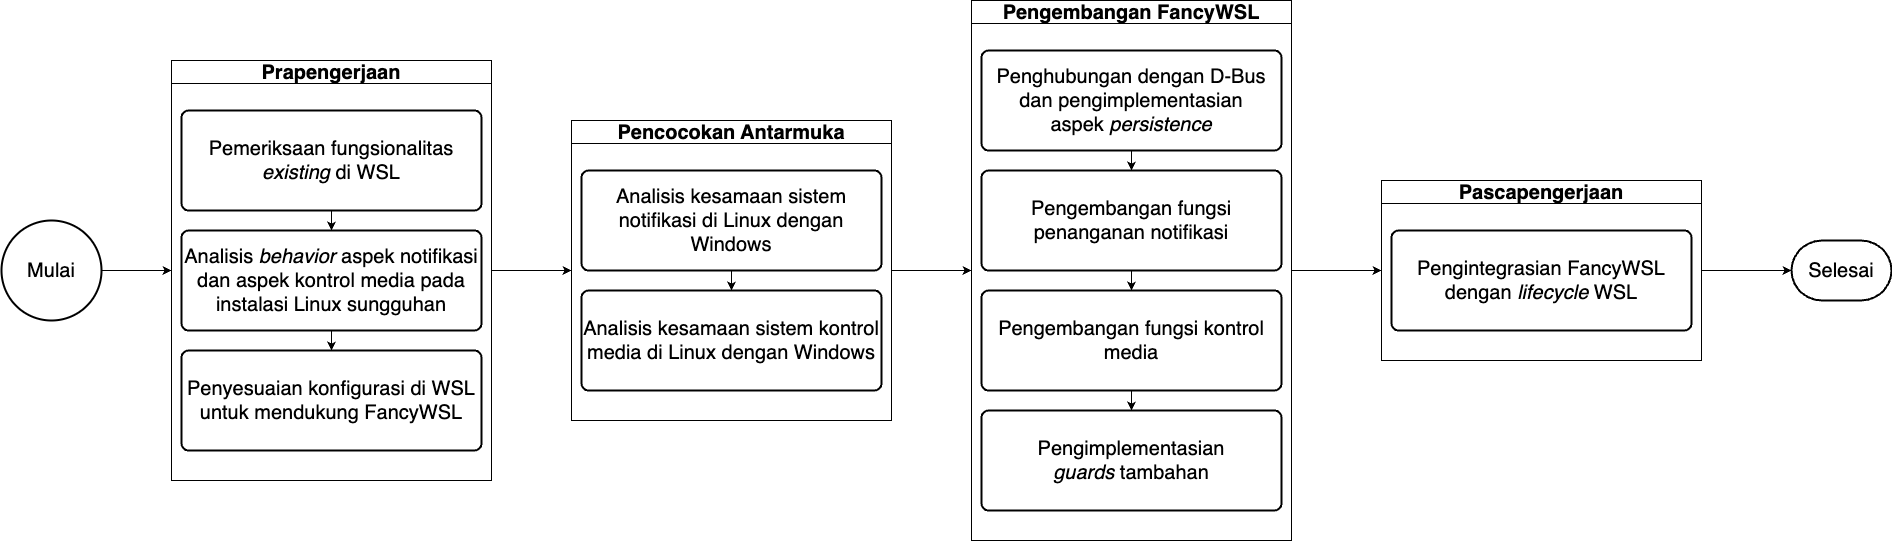
\includegraphics[width=1\linewidth]{assets/alur-pengerjaan-v1.png}
    \caption{Diagram alir (\textit{flowchart}) pelaksanaan tugas akhir}
    \label{diagram-alir-pelaksanaan}
\end{figure}

\begin{table}
    \centering
    \caption{Agenda pelaksanaan tugas akhir per minggu (\textit{week})}
    \begin{tabular}{|c|p{4cm}|c|c|c|c|c|c|c|c|} \hline 
        \multirow{3}{*}{\textbf{No.}} & \multirow{3}{*}{\textbf{Tahap}} & \multicolumn{8}{c|}{\textbf{2023}}\\ \cline{3-10} 
        & & \multicolumn{4}{c|}{\textbf{Oktober}} & \multicolumn{4}{c|}{\textbf{November}}\\ \cline{3-10} 
        & & \textbf{W1} & \textbf{W2} & \textbf{W3} & \textbf{W4} & \textbf{W1} & \textbf{W2} & \textbf{W3} & \textbf{W4}\\ \hline 
        1 & Pemeriksaan fungsionalitas di WSL & \cellcolor{black} &  &  &  &  &  &  & \\ \hline 
        2 & Analisis pada sistem operasi Linux sungguhan & \cellcolor{black} & \cellcolor{black} &  &  &  &  &  & \\ \hline 
        3 & Penyesuaian konfigurasi WSL untuk mendukung perangkat lunak FancyWSL &  &  & \cellcolor{black} & \cellcolor{black} &  &  &  & \\ \hline 
        4 & Analisis kesamaan antarmuka notifikasi &  &  & \cellcolor{black} & \cellcolor{black} & \cellcolor{black} & &  & \\ \hline 
        5 & Analisis kesamaan antarmuka pengontrolan media &  &  & \cellcolor{black} & \cellcolor{black} & \cellcolor{black} &  &  & \\ \hline 
        6 & Pengembangan perangkat lunak FancyWSL &  &  &  &  & \cellcolor{black} & \cellcolor{black} & \cellcolor{black} & \cellcolor{black}\\ \hline 
        7 & Pengintegrasian FancyWSL dengan \textit{lifecycle} WSL &  &  &  &  &  &  &  & \cellcolor{black}\\ \hline 
    \end{tabular}
    \label{tabel-agenda-pelaksanaan}
\end{table}

\section{Metode yang Digunakan}

Sesuai dengan analisis perbandingan metode yang telah dibahas di Bab II, tugas akhir ini menggunakan metode penghubungan lingkungan Windows Subsystem for Linux (WSL) dengan lingkungan \textit{host} Windows dengan memperluas cakupan koneksi bus perpesanan D-Bus yang berjalan di dalam WSL sehingga dapat dicapai oleh perangkat lunak FancyWSL yang berjalan di sisi Windows. Oleh karena itu, secara garis besar, metode tugas akhir ini dilakukan adalah dengan
\begin{enumerate}
    \item mengembangkan satu buah perangkat lunak bernama FancyWSL yang berjalan di lingkungan \textit{host} Windows dan
    \item melakukan sejumlah konfigurasi yang diperlukan di Windows Subsystem for Linux (WSL) agar dapat terhubung dengan perangkat lunak yang dikembangkan pada poin (1).
\end{enumerate}

\section{Metode Analisis Data}

Proses pengimplementasian akan dilakukan berdasarkan standar dan spesifikasi teknologi-teknokogi yang digunakan dalam tugas akhir ini. Sebagai contoh, pengimplementasian mekanisme komunikasi dengan D-Bus dilakukan dengan mengacu pada spesifikasi D-Bus \cite{dbus-specification}, pengimplementasian kapabilitas penanganan notifikasi dilakukan dengan mengacu pada FreeDesktop Desktop Notifications Specification \cite{xdg-desktop-notifications-specification}, dan pengimplementasian kapabilitas kontrol media dilakukan dengan mengacu pada standar Media Player Remote Interfacing Specification (MPRIS) \cite{xdg-mpris-specification}.

Pada akhir penelitian, akan dilakukan pengujian akhir yang membandingkan kondisi penggunaan Windows Subsystem for Linux (WSL) tanpa solusi yang dikembangkan di tugas akhir ini (kondisi bawaan) dan dengan solusi yang dikembangkan di tugas akhir ini (kondisi telah dilengkapi dengan perangkat lunak FancyWSL serta konfigurasi-konfigurasi yang diperlukan). Kedua bagian pengujian ini akan dilakukan menggunakan set perangkat lunak yang sama, yakni
\begin{itemize}
    \item Spotify (pengujian kontrol media dan notifikasi) dan
    \item Google Chrome (pengujian notifikasi).
\end{itemize}

\chapter{Hasil dan Pembahasan}

\section{Analisis pada Sistem Operasi Linux Sungguhan}

Dengan bantuan perangkat lunak virtualisasi UTM, analisis sistem penanganan notifikasi dan sisten kontrol media pada sistem operasi Linux sungguhan dilakukan pada sebuah \textit{virtual machine} (bertindak sebagai komputer referensi) yang menjalankan sistem operasi Ubuntu 22.04 (LTS) edisi arsitektur ARM 64-bit dan berjalan di atas perangkat komputer \textit{host} MacBook Air keluaran tahun 2020 (berprosesor M1) bersistem operasi macOS 13 "Ventura".

\begin{figure}[h]
    \centering
    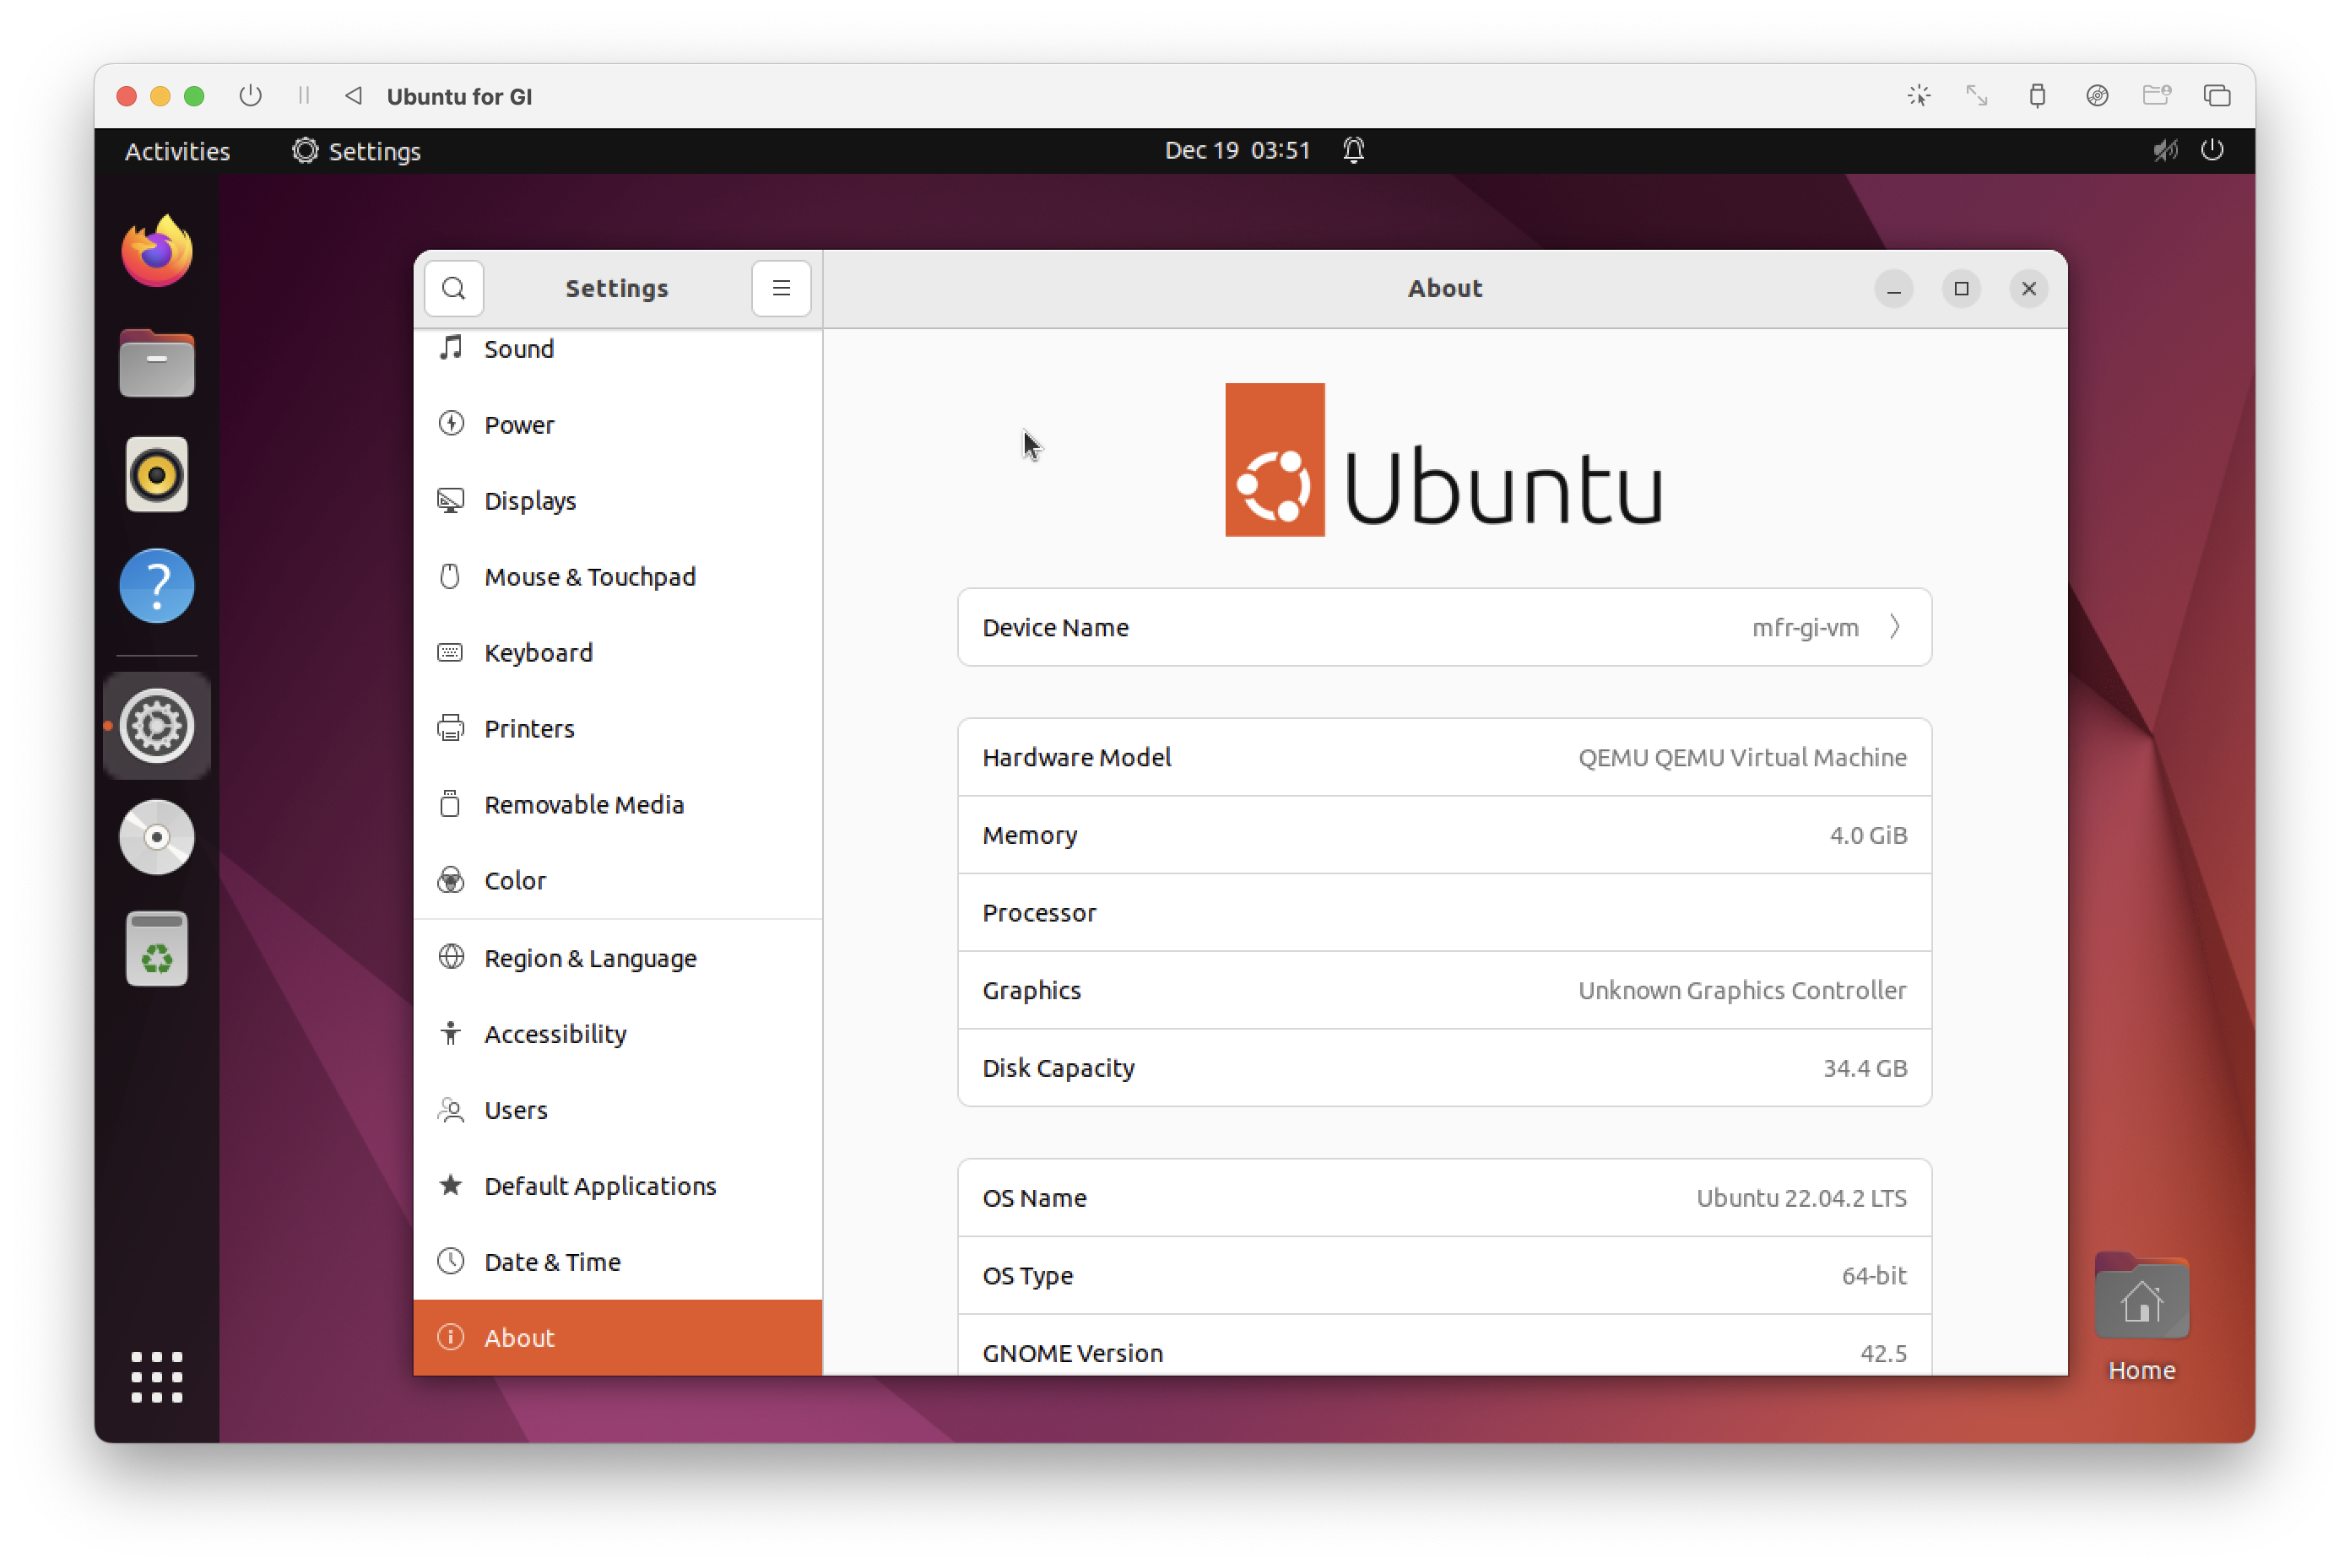
\includegraphics[width=0.75\linewidth]{archives//contents-template-pak-prapto//chapter-4/Screenshot 2023-12-19 at 10.51.04.png}
    \caption{Tangkapan layar \textit{virtual machine} Ubuntu 22.04 (LTS) yang sedang berjalan di perangkat lunak virtualisasi UTM}
    \label{fig:enter-label}
\end{figure}

\subsection{Analisis Sistem Penanganan Notifikasi}

Pengelolaan sistem penanganan notifikasi pada sistem operasi Linux bergantung pada distribusi dan/atau lingkungan desktop (\textit{desktop environment}) yang digunakan, tetapi hampir seluruh implementasi penanganan notifikasi pada sistem operasi Linux berkomunikasi melalui bus perpesanan D-Bus. Sebagai contoh, distribusi Linux yang menggunakan lingkungan \textit{desktop} GNOME menyerahkan pengelolaan notifikasi kepada \textit{desktop} GNOME itu sendiri. Uji coba sistem notifikasi pada Linux dapat dilakukan melalui berbagai cara, seperti
\begin{itemize}
    \item menggunakan perangkat lunak yang normalnya mengirimkan notifikasi (aplikasi \textit{e-mail}, aplikasi perpesanan, dan lain-lain),
    \item mensimulasikan pemanggilan metode (\textit{method}) objek D-Bus khusus yang bertugas menangani notifikasi dengan menggunakan alat (\textit{tool}) pengujian \verb|dbus-send| yang disediakan oleh paket perangkat lunak D-Bus itu sendiri, dan
    \item menggunakan alat (\textit{tool}) \verb|notify-send| yang memiliki fungsi tunggal mengirimkan notifikasi pada \textit{desktop} Linux.
\end{itemize}

Karena kepraktisannya, digunakan alat (\textit{tool}) \verb|notify-send| dalam pengujian awal ini. Alat \verb|notify-send| tersedia secara bawaan pada banyak distribusi Linux seperti Ubuntu dan Fedora. Mengutip halaman manual alat \verb|notify-send| \cite{notify-send-man-page}, alat ini dipanggil dengan bentuk pemanggilan
\begin{lstlisting}[language=bash]
    notify-send [options] {summary} [body]
\end{lstlisting}
dengan dua buah argumen utama:
\begin{itemize}
    \item argumen opsional "\textit{summary}" yang akan tertampil sebagai "judul" notifikasi dan
    \item argumen wajib "\textit{body}" yang berisi konten utama notifikasi dalam bentuk teks.
\end{itemize}
Di samping itu, alat ini juga dapat dipanggil dengan mengikutkan beberapa opsi (\textit{options}) opsional yang berkaitan dengan penampilan notifikasi:
\begin{itemize}
    \item "\verb|-u [tingkat-urgensi]|" atau "\verb|--urgency=[tingkat-urgensi]|" yang menentukan tingkat urgensi notifikasi yang akan ditampilkan (\verb|low|, \verb|normal|, atau \verb|critical|),
    \item "\verb|-t [waktu-kadaluarsa]|" atau "\verb|--expire-time=[waktu-kadaluarsa]|" yang mengatur durasi waktu notifikasi yang tertampil akan menghilang dengan sendirinya (dalam satuan milidetik),
    \item "\verb|-i [lokasi-berkas-ikon]|" atau "\verb|--icon=[lokasi-berkas-ikon]|" yang mengatur ikon yang akan ikut ditampilkan dalam notifikasi,
    \item "\verb|-c [kategori]|" atau "\verb|--category=[kategori]|" yang mengatur kategori notifikasi yang akan tertampil, dan
    \item "\verb|-h [hint]|" atau "\verb|--hint=[hint]|" yang mengatur nilai-nilai \textit{hint} untuk notifikasi yang akan tertampil.
\end{itemize}

Dalam pengujian ini, akan dikirimkan sampel notifikasi sederhana yang hanya memuat judul "Percobaan Notifikasi" dan isi pesan "Halo! Perkenalkan, nama saya Farrel.". Bentuk pemanggilan perintah \verb|notify-send| menjadi seperti berikut.
\begin{lstlisting}[language=bash]
    notify-send "Percobaan Notifikasi" "Halo! Perkenalkan, nama saya Farrel."
\end{lstlisting}
Setelah perintah tersebut dijalankan, muncul notifikasi pada layar komputer seperti pada gambar \ref{ubuntu-notify-send-demo}. Karena Ubuntu (salah satu distribusi Linux) menggunakan lingkungan desktop GNOME, penampilan notifikasi mengikuti gaya penampilan notifikasi pada lingkungan \textit{desktop} GNOME, yaitu di atas layar. Setelah beberapa saat (bergantung pada tingkat urgensi yang telah ditentukan pada pemanggilan perintah \verb|notify-send|), notifikasi akan menghilang dengan sendirinya dan masuk ke panel notifikasi yang disediakan oleh \textit{desktop} GNOME seperti pada gambar \ref{ubuntu-notification-panel}.

\begin{figure}
    \centering
    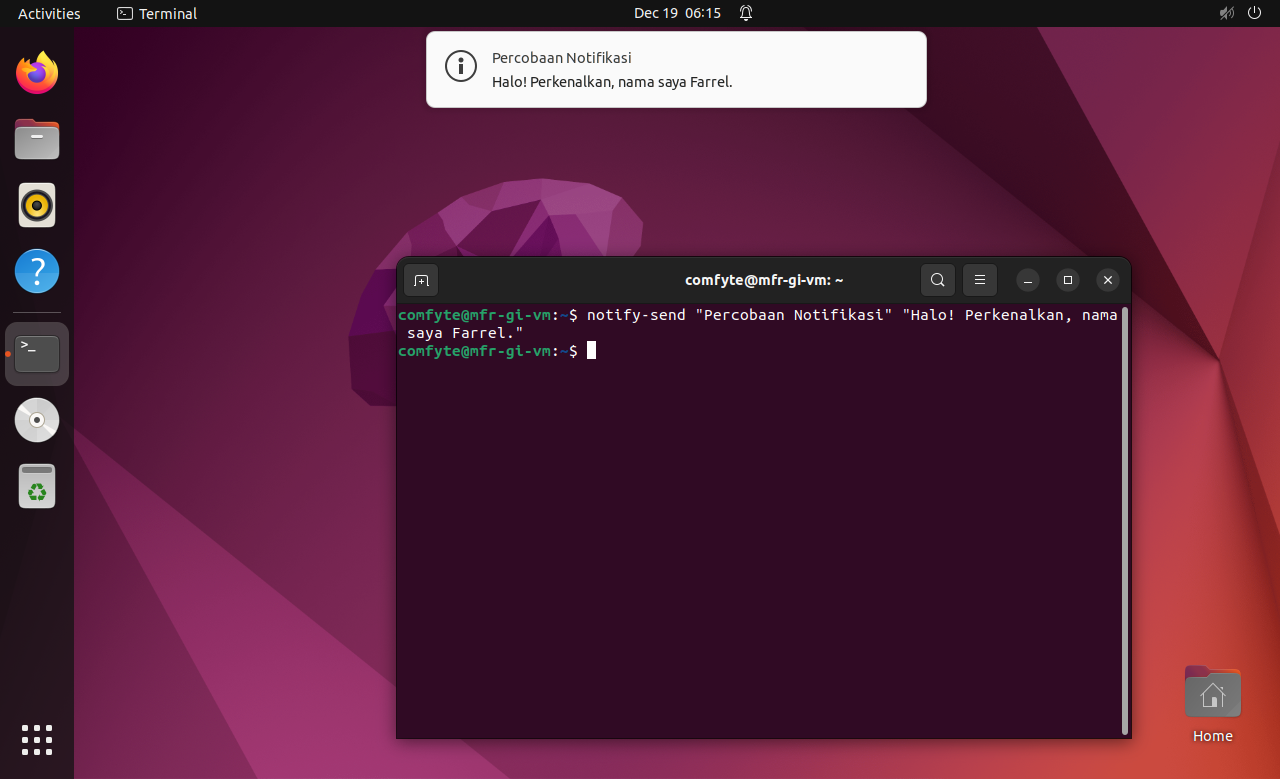
\includegraphics[width=1\linewidth]{archives//contents-template-pak-prapto//chapter-4/Screenshot from 2023-12-19 06-15-10.png}
    \caption{Notifikasi dari notify-send yang berhasil tertampil di \textit{desktop} GNOME di Ubuntu}
    \label{ubuntu-notify-send-demo}
\end{figure}

\begin{figure}
    \centering
    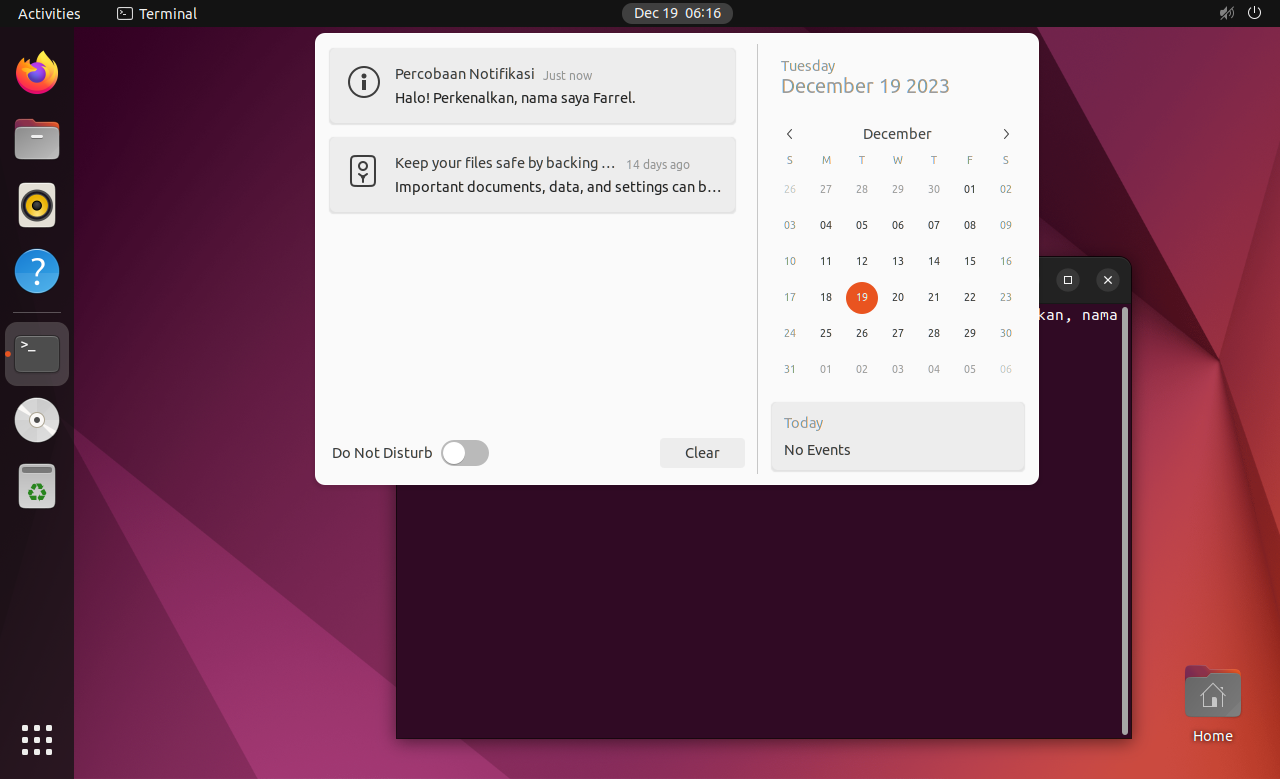
\includegraphics[width=1\linewidth]{archives//contents-template-pak-prapto//chapter-4/Screenshot from 2023-12-19 06-16-29.png}
    \caption{Panel notifikasi di \textit{desktop} GNOME yang mengumpulkan notifikasi-notifikasi lampau yang pernah tertampil}
    \label{ubuntu-notification-panel}
\end{figure}

Pada sistem operasi Linux, dimungkinkan penampilan notifikasi yang lebih kompleks (seperti mengandung tombol-tombol aksi) daripada sekadar notifikasi simpel seperti yang telah diujicobakan. Namun, mengingat alat \verb|notify-send| tidak mendukung jenis notifikasi kompleks seperti itu, pengujian pada bagian ini hanya mengujikan notifikasi yang simpel saja.

\begin{figure}
    \centering
    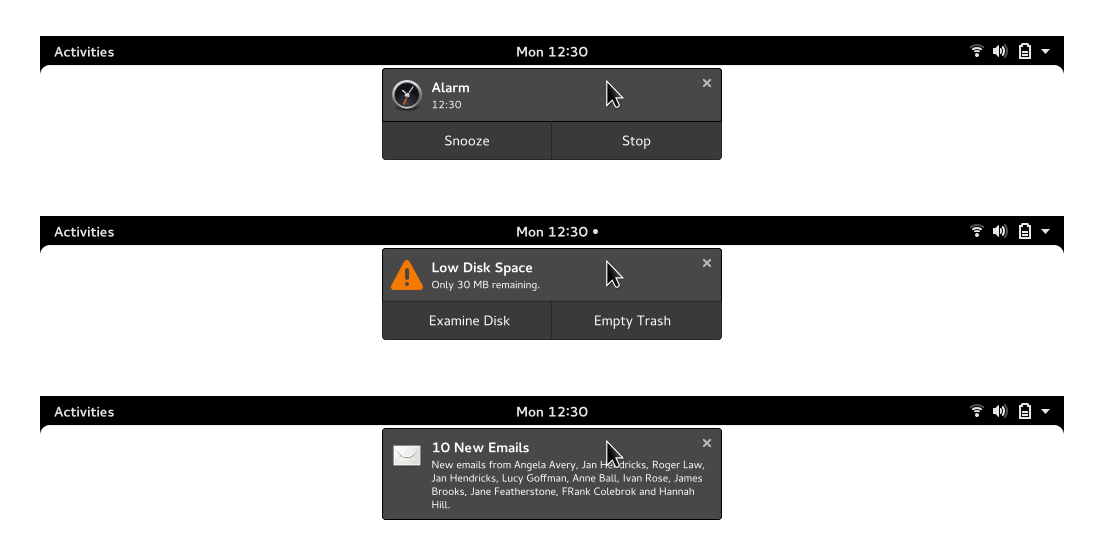
\includegraphics[width=1\linewidth]{archives//contents-template-pak-prapto//chapter-4/banners-expanded.png}
    \caption{Contoh penampilan berbagai jenis notifikasi pada lingkungan \textit{desktop} GNOME \cite{gnome-hig-notifications}; pada \textit{desktop} GNOME, notifikasi kompleks yang memiliki tombol-tombol aksi hanya akan menampilkan tombol-tombol aksi tersebut pada saat notifikasi tersebut berada di bawah kursor \textit{mouse}.}
    \label{example-of-notification-with-action-buttons-on-gnome-desktop}
\end{figure}

Di balik layar, notifikasi yang tertampil tersebut disalurkan dari \verb|notify-send| ke \textit{shell} GNOME melalui bus perpesanan D-Bus yang berjalan pada sesi (\textit{session}) pengguna saat ini. Alat \verb|notify-send| terhubung dengan bus sesi sebagai klien yang memanggil metode \verb|Notify()| pada antarmuka \verb|org.freedesktop.Notifications|; antarmuka tersebut disediakan oleh perangkat lunak \textit{notification server} yang pada lingkungan \textit{desktop} GNOME merupakan \textit{shell} GNOME itu sendiri.

Dalam serangkaian peralatan yang disediakan secara bawaan oleh paket perangkat lunak D-Bus, terdapat alat bernama \verb|dbus-monitor| yang berfungsi memantau detail pesan-pesan yang dipertukarkan di dalam bus perpesanan D-Bus. Secara \textit{default}, penjalanan \verb|dbus-monitor| tanpa memberikan argumen apa pun akan memonitor dan mencetak (di \textit{standard output}) seluruh pesan yang dipertukarkan di bus perpesanan D-Bus sehingga mungkin dirasa berlebihan; penjalanan \verb|dbus-monitor| dapat diatur dengan sebuah argumen berupa perintah filter sehingga pesan-pesan yang dimonitor dan dicetak terbatas pada pesan-pesan yang diinginkan saja. Apabila alat \verb|dbus-monitor| dijalankan dengan perintah lengkap
\begin{lstlisting}[language=bash]
    dbus-monitor "path='/org/freedesktop/Notifications'"
\end{lstlisting}
untuk memulai proses pemantauan dan perintah pengiriman notifikasi yang menggunakan \verb|notify-send| di atas dijalankan ulang, jendela terminal tempat penjalanan \verb|dbus-monitor| akan mengeluarkan informasi seperti berikut.
\begin{lstlisting}
method call time=1702972516.257275 sender=:1.48 -> destination=:1.35 serial=31 path=/org/freedesktop/Notifications; interface=org.freedesktop.Notifications; member=Notify
   string "notify-send"
   uint32 0
   string ""
   string "Percobaan Notifikasi"
   string "Halo! Perkenalkan, nama saya Farrel."
   array [
   ]
   array [
      dict entry(
         string "urgency"
         variant             byte 1
      )
      dict entry(
         string "sender-pid"
         variant             uint32 3347
      )
   ]
   int32 -1
\end{lstlisting}

Keluaran (\textit{output}) penjalanan perintah \verb|dbus-monitor| secara gamblang menunjukkan informasi-informasi teknis pada suatu penampilan notifikasi di \textit{desktop} Linux. Di samping dokumen spesifikasi resmi penanganan notifikasi di Linux sebagai acuan utama \cite{xdg-desktop-notifications-specification}, hasil keluaran alat-alat seperti \verb|dbus-monitor| dapat sangat bermanfaat untuk menginspeksi dan men-\textit{debug} mekanisme penanganan notifikasi pada tahap-tahap pengembangan yang dilakukan selanjutnya.

\subsection{Analisis Sistem Kontrol Media}

Sistem-sistem operasi modern menawarkan antarmuka pengontrolan yang mudah (umumnya berbentuk panel) saat pengguna memulai pemutaran media, baik musik, video, maupun jenis media lainnya; sistem operasi Linux pun tidak berbeda. Sistem operasi Linux menawarkan akses cepat untuk mengontrol media yang sedang diputar dengan peletakan spesifik yang menyesuaikan lingkungan \textit{desktop} yang digunakan, tetapi dengan protokol dan antarmuka yang seragam antarimplementasi tersebut. Protokol dan antarmuka yang dimaksud bernama Media Player Remote Interfacing Specification (MPRIS).



\section{Analisis Ekosistem pada Masing-Masing Platform (Linux dan Windows)}

\subsection{Analisis Sistem Penanganan Notifikasi}

\subsection{Analisis Sistem Kontrol Media}

\section{Pengembangan Perangkat Lunak FancyWSL}

\section{Perbandingan Hasil Penelitian dengan Hasil Terdahulu}

\chapter{Tambahan (Opsional)}

Anda boleh menambahkan Bab jika diperlukan. Jumlah Bab tidak harus sesuai dengan \textit{template}. 


%======================================

%======================================
%  References
%======================================
\thereferences
% You can change 
%    the filename and location of the files inputted
\bibliography{contents/references}

%======================================

%======================================
%  Appendix
%======================================
% You can change 
%    the filename and location of the files inputted
%    use \chapterappendix for the first page of the appendix
%    use \chapterappendixadd for the next page

\appendix


\chapterappendix{contents/appendices/appendix-isi-lampiran}

%======================================

\end{document}
